\documentclass{article}
\usepackage{blindtext}
\usepackage{booktabs}
\usepackage[margin=0.25in]{geometry}
\usepackage{subcaption}
\usepackage{graphicx}
\usepackage{caption}
\usepackage{hyperref}
\usepackage{pdflscape}
\usepackage{tikz}
\usepackage{threeparttable}
\usepackage{algorithmic}


\title{Simple Tables for Municipality Proliferation}

\begin{document}
\maketitle
\tableofcontents
{\footnotesize 
\listoffigures
\listoftables}
\clearpage



\section{TABLES}

\section{Balance Tables}

\begin{table}[htbp]\centering 
 \begin{threeparttable} \caption{Balance Table, Old}
 \begin{tabular}{l*{1}{c}} \toprule
                &\multicolumn{1}{c}{$\widehat{GM}$}\\
\midrule
Share population urban&    0.051** \\
                &  (0.022)   \\
\addlinespace
Fraction of area incorporated&    0.034** \\
                &  (0.017)   \\
\addlinespace
1920 transportation cost&   -0.091*  \\
                &  (0.050)   \\
\addlinespace
Coastal CZ      &    0.012   \\
                &  (0.019)   \\
\addlinespace
Fraction of urban population living in largest city&    0.012   \\
                &  (0.014)   \\
\addlinespace
Average precipitation&    0.208   \\
                &  (0.567)   \\
\addlinespace
Average temperature&   -1.524   \\
                &  (1.740)   \\
       \bottomrule \end{tabular}

{\caption*{\begin{scriptsize} Each coefficient comes from a separate regression of the baseline covariate on the instrument, controlling for census region fixed effects that Black migrants from 35 to 39 control, weighted by 1940 urban population (mirroring the main specification). \(p<0.10\), ** \(p<0.05\), *** \(p<0.01\)\end{scriptsize}}} \end{threeparttable} \label{tab:balance} \end{table}
\clearpage


\begin{table}[htbp]\centering 
 \begin{threeparttable} \caption{Balance Table, Updated}
 \begin{tabular}{l*{1}{c}} \toprule
                &\multicolumn{1}{c}{$\widehat{GM}$}\\
\midrule
Share population urban&    0.051** \\
                &  (0.022)   \\
\addlinespace
Fraction of area incorporated&    0.034** \\
                &  (0.017)   \\
\addlinespace
1920 transportation cost&   -0.091*  \\
                &  (0.050)   \\
\addlinespace
Coastal CZ      &    0.012   \\
                &  (0.019)   \\
\addlinespace
Fraction of urban population living in largest city&    0.012   \\
                &  (0.014)   \\
\addlinespace
Average precipitation&    0.208   \\
                &  (0.567)   \\
\addlinespace
Average temperature&   -1.524   \\
                &  (1.740)   \\
       \bottomrule \end{tabular}

{\caption*{\begin{scriptsize} Each coefficient comes from a separate regression of the baseline covariate on the instrument, controlling for census region fixed effects that Black migrants from 35 to 39 control, weighted by 1940 urban population (mirroring the main specification). \(p<0.10\), ** \(p<0.05\), *** \(p<0.01\)\end{scriptsize}}} \end{threeparttable} \label{tab:balance} \end{table}
\clearpage

\section{Pre-Trends}

\begin{table}[htbp]\centering 
\begin{threeparttable} \caption{Pretrends, Old}
\label{tab:pretrends}
 \begin{tabular}{l*{2}{c}} \toprule
                &\multicolumn{1}{c}{IV}&\multicolumn{1}{c}{Reduced Form}\\
\midrule
New municipalities per capita, 1900-10&   -0.005   &   -0.016   \\
                &  (0.004)   &  (0.013)   \\
\addlinespace
New municipalities per capita, 1910-20&   -0.003   &   -0.010   \\
                &  (0.005)   &  (0.018)   \\
\addlinespace
New municipalities per capita, 1920-30&    0.000   &    0.001   \\
                &  (0.002)   &  (0.007)   \\
\addlinespace
New municipalities per capita, 1930-40&   -0.001   &   -0.004   \\
                &  (0.004)   &  (0.016)   \\
\addlinespace
New municipalities per capita, 1910-40&   -0.003   &   -0.012   \\
                &  (0.008)   &  (0.031)   \\
       \bottomrule \end{tabular}

{\caption*{\begin{scriptsize} Each coefficient comes from a separate regression of the pre-period differenced outcome in IV or reduced form, controlling for census region fixed effects that Black migrants from 35 to 39 control, weighted by 1940 urban population (mirroring the main specification). \(p<0.10\), ** \(p<0.05\), *** \(p<0.01\)\end{scriptsize}}} \end{threeparttable}
\end{table}
\clearpage


\begin{table}[htbp]\centering 
\begin{threeparttable} \caption{Pretrends, Updated}
\label{tab:pretrends}
 \begin{tabular}{l*{2}{c}} \toprule
                &\multicolumn{1}{c}{IV}&\multicolumn{1}{c}{Reduced Form}\\
\midrule
New municipalities per capita, 1900-10&   -0.005   &   -0.018   \\
                &  (0.003)   &  (0.012)   \\
\addlinespace
New municipalities per capita, 1910-20&   -0.003   &   -0.011   \\
                &  (0.005)   &  (0.018)   \\
\addlinespace
New municipalities per capita, 1920-30&    0.000   &    0.001   \\
                &  (0.002)   &  (0.008)   \\
\addlinespace
New municipalities per capita, 1930-40&    0.003*  &    0.009*  \\
                &  (0.002)   &  (0.005)   \\
\addlinespace
New municipalities per capita, 1910-40&   -0.000   &   -0.001   \\
                &  (0.008)   &  (0.028)   \\
       \bottomrule \end{tabular}

{\caption*{\begin{scriptsize} Each coefficient comes from a separate regression of the pre-period differenced outcome in IV or reduced form, controlling for census region fixed effects that Black migrants from 35 to 39 control, weighted by 1940 urban population (mirroring the main specification). \(p<0.10\), ** \(p<0.05\), *** \(p<0.01\)\end{scriptsize}}} \end{threeparttable}
\end{table}
\clearpage

\begin{table}[htbp]\centering 
\begin{threeparttable} \caption{Pretrends, with Balanced controls, Old}
 \begin{tabular}{l*{2}{c}} \toprule
                &\multicolumn{1}{c}{IV}&\multicolumn{1}{c}{Reduced Form}\\
\midrule
New municipalities per capita, 1900-10&   -0.001   &   -0.004   \\
                &  (0.004)   &  (0.012)   \\
\addlinespace
New municipalities per capita, 1910-20&   -0.005   &   -0.014   \\
                &  (0.007)   &  (0.024)   \\
\addlinespace
New municipalities per capita, 1920-30&   -0.001   &   -0.004   \\
                &  (0.003)   &  (0.009)   \\
\addlinespace
New municipalities per capita, 1930-40&   -0.007*  &   -0.020   \\
                &  (0.004)   &  (0.013)   \\
\addlinespace
New municipalities per capita, 1910-40&   -0.013   &   -0.038   \\
                &  (0.012)   &  (0.041)   \\
       \bottomrule \end{tabular}

{\caption*{\begin{scriptsize} Each coefficient comes from a separate regression of the pre-period differenced outcome in IV or reduced form, controlling for census region fixed effects that Black migrants from 35 to 39 control, weighted by 1940 urban population and including the imabalnced covariates. \(p<0.10\), ** \(p<0.05\), *** \(p<0.01\)\end{scriptsize}}} \end{threeparttable}
\end{table}


\begin{table}[htbp]\centering 
\begin{threeparttable} \caption{Pretrends, with Balanced controls, Updated}
 \begin{tabular}{l*{2}{c}} \toprule
                &\multicolumn{1}{c}{IV}&\multicolumn{1}{c}{Reduced Form}\\
\midrule
New municipalities per capita, 1900-10&   -0.009*  &   -0.011   \\
                &  (0.005)   &  (0.007)   \\
\addlinespace
New municipalities per capita, 1910-20&    0.002   &    0.003   \\
                &  (0.005)   &  (0.006)   \\
\addlinespace
New municipalities per capita, 1920-30&    0.004   &    0.004   \\
                &  (0.003)   &  (0.004)   \\
\addlinespace
New municipalities per capita, 1930-40&    0.002   &    0.003   \\
                &  (0.003)   &  (0.003)   \\
\addlinespace
New municipalities per capita, 1910-40&    0.008   &    0.010   \\
                &  (0.009)   &  (0.011)   \\
       \bottomrule \end{tabular}

{\caption*{\begin{scriptsize} Each coefficient comes from a separate regression of the pre-period differenced outcome in IV or reduced form, controlling for census region fixed effects that Black migrants from 35 to 39 control, weighted by 1940 urban population and including the imabalnced covariates. \(p<0.10\), ** \(p<0.05\), *** \(p<0.01\)\end{scriptsize}}} \end{threeparttable}
\end{table}
\clearpage
\subsection{Main Effect}

\begin{table}[htbp]\centering \def\sym#1{\ifmmode^{#1}\else\(^{#1}\)\fi}  \begin{threeparttable} \caption{Effects of change in Black Migration on Municipal Proliferation, Old}
 \begin{tabular}{l*{8}{c}} \toprule
&\multicolumn{1}{c}{C. Goodman}&\multicolumn{4}{c}{Census of Governments}&\multicolumn{1}{c}{Census}\\\cmidrule(lr){2-2}\cmidrule(lr){3-6}\cmidrule(lr){7-7}
&\multicolumn{2}{c}{Municipalities}&\multicolumn{1}{c}{School districts}&\multicolumn{1}{c}{Townships}&\multicolumn{1}{c}{Special districts}&\multicolumn{1}{c}{Principal City Share}\\\cmidrule(lr){2-3}\cmidrule(lr){4-6}\cmidrule(lr){7-7}
&\multicolumn{1}{c}{(1)}&\multicolumn{1}{c}{(2)}&\multicolumn{1}{c}{(3)}&\multicolumn{1}{c}{(4)}&\multicolumn{1}{c}{(5)}&\multicolumn{1}{c}{(6)}\\
\cmidrule(lr){1-7}
\multicolumn{6}{l}{Panel A: First Stage}\\
\cmidrule(lr){1-7}
$\widehat{GM}$  &    3.464***&    3.464***&    3.464***&    3.464***&    3.464***&    3.464***\\
                &  (0.418)   &  (0.418)   &  (0.418)   &  (0.418)   &  (0.418)   &  (0.418)   \\
\cmidrule(lr){1-7}
\multicolumn{6}{l}{Panel B: OLS}\\
\cmidrule(lr){1-7}
GM              &    0.006*  &    0.009** &    0.288***&    0.016***&   -0.027***&   -0.810***\\
                &  (0.004)   &  (0.004)   &  (0.084)   &  (0.005)   &  (0.008)   &  (0.267)   \\
\cmidrule(lr){1-7}
\multicolumn{6}{l}{Panel C: Reduced Form}\\
\cmidrule(lr){1-7}
$\widehat{GM}$  &    0.040*  &    0.053** &    1.446***&    0.104***&   -0.076** &   -4.232***\\
                &  (0.023)   &  (0.025)   &  (0.423)   &  (0.030)   &  (0.032)   &  (1.500)   \\
\cmidrule(lr){1-7}
\multicolumn{6}{l}{Panel D: 2SLS}\\
\cmidrule(lr){1-7}
GM              &    0.011*  &    0.015** &    0.418***&    0.030***&   -0.022** &   -1.222***\\
                &  (0.006)   &  (0.007)   &  (0.115)   &  (0.008)   &  (0.009)   &  (0.398)   \\
\midrule
First Stage F-Stat&    68.63   &    68.63   &    68.63   &    68.63   &    68.63   &    68.63   \\
Dependent Variable Mean&     -.17   &      -.2   &    -3.58   &     -.25   &      .26   &   -17.07   \\
Observations    &      130   &      130   &      130   &      130   &      130   &      130   \\
       \bottomrule \end{tabular}

{\caption*{\begin{scriptsize} "\(p<0.10\), ** \(p<0.05\), *** \(p<0.01\)"\end{scriptsize}}} \end{threeparttable} \end{table}
\clearpage


\begin{table}[htbp]\centering \def\sym#1{\ifmmode^{#1}\else\(^{#1}\)\fi}  \begin{threeparttable} \caption{Effects of change in Black Migration on Municipal Proliferation, Updated}
 \begin{tabular}{l*{8}{c}} \toprule
&\multicolumn{1}{c}{C. Goodman}&\multicolumn{4}{c}{Census of Governments}&\multicolumn{1}{c}{Census}\\\cmidrule(lr){2-2}\cmidrule(lr){3-6}\cmidrule(lr){7-7}
&\multicolumn{2}{c}{Municipalities}&\multicolumn{1}{c}{School districts}&\multicolumn{1}{c}{Townships}&\multicolumn{1}{c}{Special districts}&\multicolumn{1}{c}{Main City Share}\\\cmidrule(lr){2-3}\cmidrule(lr){4-6}\cmidrule(lr){7-7}
&\multicolumn{1}{c}{(1)}&\multicolumn{1}{c}{(2)}&\multicolumn{1}{c}{(3)}&\multicolumn{1}{c}{(4)}&\multicolumn{1}{c}{(5)}&\multicolumn{1}{c}{(6)}\\
\cmidrule(lr){1-7}
\multicolumn{6}{l}{Panel A: First Stage}\\
\cmidrule(lr){1-7}
$\widehat{GM}$  &    1.399***&    1.399***&    1.399***&    1.399***&    1.399***&    1.399***\\
                &  (0.233)   &  (0.233)   &  (0.233)   &  (0.233)   &  (0.233)   &  (0.233)   \\
\cmidrule(lr){1-7}
\multicolumn{6}{l}{Panel B: OLS}\\
\cmidrule(lr){1-7}
GM              &    0.004   &    0.008** &    0.304***&    0.017***&   -0.027***&   -1.099***\\
                &  (0.003)   &  (0.004)   &  (0.091)   &  (0.006)   &  (0.009)   &  (0.147)   \\
\cmidrule(lr){1-7}
\multicolumn{6}{l}{Panel C: Reduced Form}\\
\cmidrule(lr){1-7}
$\widehat{GM}$  &    0.010*  &    0.015** &    0.306   &    0.035***&   -0.010   &   -1.946***\\
                &  (0.006)   &  (0.007)   &  (0.194)   &  (0.011)   &  (0.015)   &  (0.293)   \\
\cmidrule(lr){1-7}
\multicolumn{6}{l}{Panel D: 2SLS}\\
\cmidrule(lr){1-7}
GM              &    0.007*  &    0.011** &    0.219*  &    0.025***&   -0.007   &   -1.391***\\
                &  (0.004)   &  (0.005)   &  (0.116)   &  (0.007)   &  (0.010)   &  (0.133)   \\
\midrule
First Stage F-Stat&    35.97   &    35.97   &    35.97   &    35.97   &    35.97   &    35.97   \\
Dep. Var. Mean  &    -0.14   &    -0.18   &    -3.64   &    -0.25   &     0.26   &   -14.58   \\
1940 Dep. Var. Mean&     0.63   &     0.68   &     4.10   &     0.81   &     0.43   &    50.06   \\
Observations    &      130   &      130   &      130   &      130   &      130   &      130   \\
       \bottomrule \end{tabular}

{\caption*{\begin{scriptsize} "\(p<0.10\), ** \(p<0.05\), *** \(p<0.01\)"\end{scriptsize}}} \end{threeparttable} \end{table}
\clearpage


\begin{table}[htbp]\centering \def\sym#1{\ifmmode^{#1}\else\(^{#1}\)\fi}  \begin{threeparttable} \caption{Effects of change in Black Migration on Municipal Proliferation, Balanced Controls, Old}
 \begin{tabular}{l*{8}{c}} \toprule
&\multicolumn{1}{c}{C. Goodman}&\multicolumn{4}{c}{Census of Governments}&\multicolumn{1}{c}{Census}\\\cmidrule(lr){2-2}\cmidrule(lr){3-6}\cmidrule(lr){7-7}
&\multicolumn{2}{c}{Municipalities}&\multicolumn{1}{c}{School districts}&\multicolumn{1}{c}{Townships}&\multicolumn{1}{c}{Special districts}&\multicolumn{1}{c}{Principal City Share}\\\cmidrule(lr){2-3}\cmidrule(lr){4-6}\cmidrule(lr){7-7}
&\multicolumn{1}{c}{(1)}&\multicolumn{1}{c}{(2)}&\multicolumn{1}{c}{(3)}&\multicolumn{1}{c}{(4)}&\multicolumn{1}{c}{(5)}&\multicolumn{1}{c}{(6)}\\
\cmidrule(lr){1-7}
\multicolumn{6}{l}{Panel A: First Stage}\\
\cmidrule(lr){1-7}
$\widehat{GM}$  &    3.260***&    3.260***&    3.260***&    3.260***&    3.260***&    3.260***\\
                &  (0.464)   &  (0.464)   &  (0.464)   &  (0.464)   &  (0.464)   &  (0.464)   \\
\cmidrule(lr){1-7}
\multicolumn{6}{l}{Panel B: OLS}\\
\cmidrule(lr){1-7}
GM              &    0.011***&    0.014***&    0.272***&    0.012** &   -0.026***&   -0.234   \\
                &  (0.004)   &  (0.004)   &  (0.081)   &  (0.005)   &  (0.007)   &  (0.144)   \\
\cmidrule(lr){1-7}
\multicolumn{6}{l}{Panel C: Reduced Form}\\
\cmidrule(lr){1-7}
$\widehat{GM}$  &    0.056***&    0.069***&    1.364***&    0.081***&   -0.063*  &   -1.837***\\
                &  (0.019)   &  (0.020)   &  (0.425)   &  (0.030)   &  (0.034)   &  (0.697)   \\
\cmidrule(lr){1-7}
\multicolumn{6}{l}{Panel D: 2SLS}\\
\cmidrule(lr){1-7}
GM              &    0.017***&    0.021***&    0.418***&    0.025***&   -0.019*  &   -0.563***\\
                &  (0.005)   &  (0.005)   &  (0.127)   &  (0.009)   &  (0.010)   &  (0.217)   \\
\midrule
First Stage F-Stat&    49.36   &    49.36   &    49.36   &    49.36   &    49.36   &    49.36   \\
Dependent Variable Mean&     -.17   &      -.2   &    -3.58   &     -.25   &      .26   &   -17.07   \\
Observations    &      130   &      130   &      130   &      130   &      130   &      130   \\
       \bottomrule \end{tabular}

{\caption*{\begin{scriptsize} "\(p<0.10\), ** \(p<0.05\), *** \(p<0.01\)"\end{scriptsize}}} \end{threeparttable} \end{table}
\clearpage



\begin{table}[htbp]\centering \def\sym#1{\ifmmode^{#1}\else\(^{#1}\)\fi}  \begin{threeparttable} \caption{Effects of change in Black Migration on Municipal Proliferation, Balanced Controls, Updated}
 \begin{tabular}{l*{8}{c}} \toprule
&\multicolumn{1}{c}{C. Goodman}&\multicolumn{4}{c}{Census of Governments}&\multicolumn{1}{c}{Census}\\\cmidrule(lr){2-2}\cmidrule(lr){3-6}\cmidrule(lr){7-7}
&\multicolumn{2}{c}{Municipalities}&\multicolumn{1}{c}{School districts}&\multicolumn{1}{c}{Townships}&\multicolumn{1}{c}{Special districts}&\multicolumn{1}{c}{Principal City Share}\\\cmidrule(lr){2-3}\cmidrule(lr){4-6}\cmidrule(lr){7-7}
&\multicolumn{1}{c}{(1)}&\multicolumn{1}{c}{(2)}&\multicolumn{1}{c}{(3)}&\multicolumn{1}{c}{(4)}&\multicolumn{1}{c}{(5)}&\multicolumn{1}{c}{(6)}\\
\cmidrule(lr){1-7}
\multicolumn{6}{l}{Panel A: First Stage}\\
\cmidrule(lr){1-7}
$\widehat{GM}$  &    3.260***&    3.260***&    3.260***&    3.260***&    3.260***&    3.260***\\
                &  (0.464)   &  (0.464)   &  (0.464)   &  (0.464)   &  (0.464)   &  (0.464)   \\
\cmidrule(lr){1-7}
\multicolumn{6}{l}{Panel B: OLS}\\
\cmidrule(lr){1-7}
GM              &    0.011***&    0.014***&    0.272***&    0.012** &   -0.026***&   -0.234   \\
                &  (0.004)   &  (0.004)   &  (0.081)   &  (0.005)   &  (0.007)   &  (0.144)   \\
\cmidrule(lr){1-7}
\multicolumn{6}{l}{Panel C: Reduced Form}\\
\cmidrule(lr){1-7}
$\widehat{GM}$  &    0.056***&    0.069***&    1.364***&    0.081***&   -0.063*  &   -1.837***\\
                &  (0.019)   &  (0.020)   &  (0.425)   &  (0.030)   &  (0.034)   &  (0.697)   \\
\cmidrule(lr){1-7}
\multicolumn{6}{l}{Panel D: 2SLS}\\
\cmidrule(lr){1-7}
GM              &    0.017***&    0.021***&    0.418***&    0.025***&   -0.019*  &   -0.563***\\
                &  (0.005)   &  (0.005)   &  (0.127)   &  (0.009)   &  (0.010)   &  (0.217)   \\
\midrule
First Stage F-Stat&    49.36   &    49.36   &    49.36   &    49.36   &    49.36   &    49.36   \\
Dependent Variable Mean&     -.17   &      -.2   &    -3.58   &     -.25   &      .26   &   -17.07   \\
Observations    &      130   &      130   &      130   &      130   &      130   &      130   \\
       \bottomrule \end{tabular}

{\caption*{\begin{scriptsize} "\(p<0.10\), ** \(p<0.05\), *** \(p<0.01\)"\end{scriptsize}}} \end{threeparttable} \end{table}
\clearpage

\subsection{Main Effect, Percentile Instrument}
\begin{table}[htbp]\centering \def\sym#1{\ifmmode^{#1}\else\(^{#1}\)\fi}  \begin{threeparttable} \caption{Effects of change in Black Migration on Municipal Proliferation, Percentile Rank, Old}
 \begin{tabular}{l*{8}{c}} \toprule
&\multicolumn{1}{c}{C. Goodman}&\multicolumn{4}{c}{Census of Governments}&\multicolumn{1}{c}{Census}\\\cmidrule(lr){2-2}\cmidrule(lr){3-6}\cmidrule(lr){7-7}
&\multicolumn{2}{c}{Municipalities}&\multicolumn{1}{c}{School districts}&\multicolumn{1}{c}{Townships}&\multicolumn{1}{c}{Special districts}&\multicolumn{1}{c}{Principal City Share}\\\cmidrule(lr){2-3}\cmidrule(lr){4-6}\cmidrule(lr){7-7}
&\multicolumn{1}{c}{(1)}&\multicolumn{1}{c}{(2)}&\multicolumn{1}{c}{(3)}&\multicolumn{1}{c}{(4)}&\multicolumn{1}{c}{(5)}&\multicolumn{1}{c}{(6)}\\
\cmidrule(lr){1-7}
\multicolumn{6}{l}{Panel A: First Stage}\\
\cmidrule(lr){1-7}
$\widehat{GM}$ Percentile&    0.639***&    0.639***&    0.639***&    0.639***&    0.639***&    0.639***\\
                &  (0.099)   &  (0.099)   &  (0.099)   &  (0.099)   &  (0.099)   &  (0.099)   \\
\cmidrule(lr){1-7}
\multicolumn{6}{l}{Panel B: OLS}\\
\cmidrule(lr){1-7}
GM Percentile   &    0.003   &    0.005** &    0.110***&    0.003*  &   -0.011***&    0.034   \\
                &  (0.002)   &  (0.002)   &  (0.028)   &  (0.002)   &  (0.003)   &  (0.149)   \\
\cmidrule(lr){1-7}
\multicolumn{6}{l}{Panel C: Reduced Form}\\
\cmidrule(lr){1-7}
$\widehat{GM}$ Percentile&    0.005** &    0.005** &    0.108***&    0.006***&   -0.004   &    0.054   \\
                &  (0.002)   &  (0.002)   &  (0.032)   &  (0.002)   &  (0.003)   &  (0.172)   \\
\cmidrule(lr){1-7}
\multicolumn{6}{l}{Panel D: 2SLS}\\
\cmidrule(lr){1-7}
GM Percentile   &    0.007** &    0.008** &    0.169***&    0.009** &   -0.006   &    0.084   \\
                &  (0.003)   &  (0.003)   &  (0.049)   &  (0.003)   &  (0.004)   &  (0.261)   \\
\midrule
First Stage F-Stat&     41.8   &     41.8   &     41.8   &     41.8   &     41.8   &     41.8   \\
Dependent Variable Mean&     -.17   &      -.2   &    -3.58   &     -.25   &      .26   &   -17.07   \\
Observations    &      130   &      130   &      130   &      130   &      130   &      130   \\
       \bottomrule \end{tabular}

{\caption*{\begin{scriptsize} "\(p<0.10\), ** \(p<0.05\), *** \(p<0.01\)"\end{scriptsize}}} \end{threeparttable} \end{table}


\begin{table}[htbp]\centering \def\sym#1{\ifmmode^{#1}\else\(^{#1}\)\fi}  \begin{threeparttable} \caption{Effects of change in Black Migration on Municipal Proliferation, Percentile Rank, Updated}
 \begin{tabular}{l*{8}{c}} \toprule
&\multicolumn{1}{c}{C. Goodman}&\multicolumn{4}{c}{Census of Governments}&\multicolumn{1}{c}{Census}\\\cmidrule(lr){2-2}\cmidrule(lr){3-6}\cmidrule(lr){7-7}
&\multicolumn{2}{c}{Municipalities}&\multicolumn{1}{c}{School districts}&\multicolumn{1}{c}{Townships}&\multicolumn{1}{c}{Special districts}&\multicolumn{1}{c}{Main City Share}\\\cmidrule(lr){2-3}\cmidrule(lr){4-6}\cmidrule(lr){7-7}
&\multicolumn{1}{c}{(1)}&\multicolumn{1}{c}{(2)}&\multicolumn{1}{c}{(3)}&\multicolumn{1}{c}{(4)}&\multicolumn{1}{c}{(5)}&\multicolumn{1}{c}{(6)}\\
\cmidrule(lr){1-7}
\multicolumn{6}{l}{Panel A: First Stage}\\
\cmidrule(lr){1-7}
$\widehat{GM}$ Percentile&    0.714***&    0.714***&    0.714***&    0.714***&    0.714***&    0.714***\\
                &  (0.084)   &  (0.084)   &  (0.084)   &  (0.084)   &  (0.084)   &  (0.084)   \\
\cmidrule(lr){1-7}
\multicolumn{6}{l}{Panel B: OLS}\\
\cmidrule(lr){1-7}
GM Percentile   &    0.001   &    0.002*  &    0.119***&    0.005***&   -0.012***&   -0.276***\\
                &  (0.001)   &  (0.001)   &  (0.026)   &  (0.002)   &  (0.003)   &  (0.044)   \\
\cmidrule(lr){1-7}
\multicolumn{6}{l}{Panel C: Reduced Form}\\
\cmidrule(lr){1-7}
$\widehat{GM}$ Percentile&    0.001*  &    0.002** &    0.115***&    0.006***&   -0.007** &   -0.263***\\
                &  (0.001)   &  (0.001)   &  (0.028)   &  (0.002)   &  (0.003)   &  (0.041)   \\
\cmidrule(lr){1-7}
\multicolumn{6}{l}{Panel D: 2SLS}\\
\cmidrule(lr){1-7}
GM Percentile   &    0.002*  &    0.003** &    0.162***&    0.009***&   -0.010***&   -0.369***\\
                &  (0.001)   &  (0.001)   &  (0.039)   &  (0.003)   &  (0.003)   &  (0.052)   \\
\midrule
First Stage F-Stat&    71.85   &    71.85   &    71.85   &    71.85   &    71.85   &    71.85   \\
Dep. Var. Mean  &    -0.14   &    -0.17   &    -3.57   &    -0.25   &     0.26   &   -14.64   \\
1940 Dep. Var. Mean&     0.63   &     0.68   &     4.03   &     0.81   &     0.42   &    50.41   \\
Observations    &      130   &      130   &      130   &      130   &      130   &      130   \\
       \bottomrule \end{tabular}

{\caption*{\begin{scriptsize} "\(p<0.10\), ** \(p<0.05\), *** \(p<0.01\)"\end{scriptsize}}} \end{threeparttable} \end{table}

\begin{table}[htbp]\centering \def\sym#1{\ifmmode^{#1}\else\(^{#1}\)\fi}  \begin{threeparttable} \caption{Effects of change in Black Migration on Municipal Proliferation, Percentile Rank, Balanced Controls, Old}
 \begin{tabular}{l*{8}{c}} \toprule
&\multicolumn{1}{c}{C. Goodman}&\multicolumn{4}{c}{Census of Governments}&\multicolumn{1}{c}{Census}\\\cmidrule(lr){2-2}\cmidrule(lr){3-6}\cmidrule(lr){7-7}
&\multicolumn{2}{c}{Municipalities}&\multicolumn{1}{c}{School districts}&\multicolumn{1}{c}{Townships}&\multicolumn{1}{c}{Special districts}&\multicolumn{1}{c}{Principal City Share}\\\cmidrule(lr){2-3}\cmidrule(lr){4-6}\cmidrule(lr){7-7}
&\multicolumn{1}{c}{(1)}&\multicolumn{1}{c}{(2)}&\multicolumn{1}{c}{(3)}&\multicolumn{1}{c}{(4)}&\multicolumn{1}{c}{(5)}&\multicolumn{1}{c}{(6)}\\
\cmidrule(lr){1-7}
\multicolumn{6}{l}{Panel A: First Stage}\\
\cmidrule(lr){1-7}
$\widehat{GM}$ Percentile&    0.639***&    0.639***&    0.639***&    0.639***&    0.639***&    0.639***\\
                &  (0.124)   &  (0.124)   &  (0.124)   &  (0.124)   &  (0.124)   &  (0.124)   \\
\cmidrule(lr){1-7}
\multicolumn{6}{l}{Panel B: OLS}\\
\cmidrule(lr){1-7}
GM Percentile   &    0.003*  &    0.004** &    0.107***&    0.001   &   -0.010***&    0.068   \\
                &  (0.002)   &  (0.002)   &  (0.027)   &  (0.002)   &  (0.002)   &  (0.042)   \\
\cmidrule(lr){1-7}
\multicolumn{6}{l}{Panel C: Reduced Form}\\
\cmidrule(lr){1-7}
$\widehat{GM}$ Percentile&    0.004***&    0.005***&    0.132***&    0.004*  &   -0.007** &   -0.004   \\
                &  (0.001)   &  (0.002)   &  (0.032)   &  (0.002)   &  (0.003)   &  (0.053)   \\
\cmidrule(lr){1-7}
\multicolumn{6}{l}{Panel D: 2SLS}\\
\cmidrule(lr){1-7}
GM Percentile   &    0.006***&    0.007***&    0.206***&    0.007*  &   -0.011***&   -0.006   \\
                &  (0.002)   &  (0.002)   &  (0.051)   &  (0.004)   &  (0.004)   &  (0.080)   \\
\midrule
First Stage F-Stat&    26.54   &    26.54   &    26.54   &    26.54   &    26.54   &    26.54   \\
Dependent Variable Mean&     -.17   &      -.2   &    -3.58   &     -.25   &      .26   &   -17.07   \\
Observations    &      130   &      130   &      130   &      130   &      130   &      130   \\
       \bottomrule \end{tabular}

{\caption*{\begin{scriptsize} "\(p<0.10\), ** \(p<0.05\), *** \(p<0.01\)"\end{scriptsize}}} \end{threeparttable} \end{table}


\begin{table}[htbp]\centering \def\sym#1{\ifmmode^{#1}\else\(^{#1}\)\fi}  \begin{threeparttable} \caption{Effects of change in Black Migration on Municipal Proliferation, Percentile Rank, Balanced Controls, Updated}
 \begin{tabular}{l*{8}{c}} \toprule
&\multicolumn{1}{c}{C. Goodman}&\multicolumn{4}{c}{Census of Governments}&\multicolumn{1}{c}{Census}\\\cmidrule(lr){2-2}\cmidrule(lr){3-6}\cmidrule(lr){7-7}
&\multicolumn{2}{c}{Municipalities}&\multicolumn{1}{c}{School districts}&\multicolumn{1}{c}{Townships}&\multicolumn{1}{c}{Special districts}&\multicolumn{1}{c}{Principal City Share}\\\cmidrule(lr){2-3}\cmidrule(lr){4-6}\cmidrule(lr){7-7}
&\multicolumn{1}{c}{(1)}&\multicolumn{1}{c}{(2)}&\multicolumn{1}{c}{(3)}&\multicolumn{1}{c}{(4)}&\multicolumn{1}{c}{(5)}&\multicolumn{1}{c}{(6)}\\
\cmidrule(lr){1-7}
\multicolumn{6}{l}{Panel A: First Stage}\\
\cmidrule(lr){1-7}
$\widehat{GM}$ Percentile&    0.626***&    0.626***&    0.626***&    0.626***&    0.626***&    0.626***\\
                &  (0.110)   &  (0.110)   &  (0.110)   &  (0.110)   &  (0.110)   &  (0.110)   \\
\cmidrule(lr){1-7}
\multicolumn{6}{l}{Panel B: OLS}\\
\cmidrule(lr){1-7}
GM Percentile   &    0.000   &    0.001   &    0.065** &    0.003   &   -0.015***&   -0.240***\\
                &  (0.001)   &  (0.001)   &  (0.027)   &  (0.002)   &  (0.002)   &  (0.049)   \\
\cmidrule(lr){1-7}
\multicolumn{6}{l}{Panel C: Reduced Form}\\
\cmidrule(lr){1-7}
$\widehat{GM}$ Percentile&    0.002** &    0.003** &    0.104***&    0.005** &   -0.009***&   -0.240***\\
                &  (0.001)   &  (0.001)   &  (0.027)   &  (0.002)   &  (0.003)   &  (0.059)   \\
\cmidrule(lr){1-7}
\multicolumn{6}{l}{Panel D: 2SLS}\\
\cmidrule(lr){1-7}
GM Percentile   &    0.003** &    0.004** &    0.167***&    0.008** &   -0.015***&   -0.383***\\
                &  (0.002)   &  (0.002)   &  (0.044)   &  (0.004)   &  (0.004)   &  (0.088)   \\
\midrule
First Stage F-Stat&    32.31   &    32.31   &    32.31   &    32.31   &    32.31   &    32.31   \\
Dependent Variable Mean&     -.14   &     -.17   &    -3.57   &     -.25   &      .26   &   -14.64   \\
Observations    &      130   &      130   &      130   &      130   &      130   &      130   \\
       \bottomrule \end{tabular}

{\caption*{\begin{scriptsize} "\(p<0.10\), ** \(p<0.05\), *** \(p<0.01\)"\end{scriptsize}}} \end{threeparttable} \end{table}
\clearpage

\subsection{Main Effect, 1950-70}

\begin{table}[htbp]\centering \def\sym#1{\ifmmode^{#1}\else\(^{#1}\)\fi}  \begin{threeparttable} \caption{Effects of change in Black Migration on Municipal Proliferation, 1950-70, Old}
 \begin{tabular}{l*{8}{c}} \toprule
&\multicolumn{1}{c}{C. Goodman}&\multicolumn{4}{c}{Census of Governments}&\multicolumn{1}{c}{Census}\\\cmidrule(lr){2-2}\cmidrule(lr){3-6}\cmidrule(lr){7-7}
&\multicolumn{2}{c}{Municipalities}&\multicolumn{1}{c}{School districts}&\multicolumn{1}{c}{Townships}&\multicolumn{1}{c}{Special districts}&\multicolumn{1}{c}{Principal City Share}\\\cmidrule(lr){2-3}\cmidrule(lr){4-6}\cmidrule(lr){7-7}
&\multicolumn{1}{c}{(1)}&\multicolumn{1}{c}{(2)}&\multicolumn{1}{c}{(3)}&\multicolumn{1}{c}{(4)}&\multicolumn{1}{c}{(5)}&\multicolumn{1}{c}{(6)}\\
\cmidrule(lr){1-7}
\multicolumn{6}{l}{Panel A: First Stage}\\
\cmidrule(lr){1-7}
$\widehat{GM}$  &    3.464***&    3.464***&    3.464***&    3.464***&    3.464***&    3.464***\\
                &  (0.418)   &  (0.418)   &  (0.418)   &  (0.418)   &  (0.418)   &  (0.418)   \\
\cmidrule(lr){1-7}
\multicolumn{6}{l}{Panel B: OLS}\\
\cmidrule(lr){1-7}
GM              &    0.004*  &    0.006** &    0.183***&    0.011***&   -0.017** &   -0.675***\\
                &  (0.002)   &  (0.002)   &  (0.050)   &  (0.003)   &  (0.007)   &  (0.195)   \\
\cmidrule(lr){1-7}
\multicolumn{6}{l}{Panel C: Reduced Form}\\
\cmidrule(lr){1-7}
$\widehat{GM}$  &    0.023*  &    0.030** &    0.919***&    0.067***&   -0.057** &   -3.705***\\
                &  (0.012)   &  (0.014)   &  (0.223)   &  (0.017)   &  (0.025)   &  (1.013)   \\
\cmidrule(lr){1-7}
\multicolumn{6}{l}{Panel D: 2SLS}\\
\cmidrule(lr){1-7}
GM              &    0.007** &    0.009** &    0.265***&    0.019***&   -0.016** &   -1.070***\\
                &  (0.003)   &  (0.003)   &  (0.061)   &  (0.004)   &  (0.007)   &  (0.258)   \\
\midrule
First Stage F-Stat&    68.63   &    68.63   &    68.63   &    68.63   &    68.63   &    68.63   \\
Dependent Variable Mean&      -.1   &     -.11   &    -1.88   &     -.16   &      .19   &   -12.88   \\
Observations    &      130   &      130   &      130   &      130   &      130   &      130   \\
       \bottomrule \end{tabular}

{\caption*{\begin{scriptsize} "\(p<0.10\), ** \(p<0.05\), *** \(p<0.01\)"\end{scriptsize}}} \end{threeparttable} \end{table}

\clearpage
\begin{table}[htbp]\centering \def\sym#1{\ifmmode^{#1}\else\(^{#1}\)\fi}  \begin{threeparttable} \caption{Effects of change in Black Migration on Municipal Proliferation, 1950-70, Updated}
 \begin{tabular}{l*{8}{c}} \toprule
&\multicolumn{1}{c}{C. Goodman}&\multicolumn{4}{c}{Census of Governments}&\multicolumn{1}{c}{Census}\\\cmidrule(lr){2-2}\cmidrule(lr){3-6}\cmidrule(lr){7-7}
&\multicolumn{2}{c}{Municipalities}&\multicolumn{1}{c}{School districts}&\multicolumn{1}{c}{Townships}&\multicolumn{1}{c}{Special districts}&\multicolumn{1}{c}{Main City Share}\\\cmidrule(lr){2-3}\cmidrule(lr){4-6}\cmidrule(lr){7-7}
&\multicolumn{1}{c}{(1)}&\multicolumn{1}{c}{(2)}&\multicolumn{1}{c}{(3)}&\multicolumn{1}{c}{(4)}&\multicolumn{1}{c}{(5)}&\multicolumn{1}{c}{(6)}\\
\cmidrule(lr){1-7}
\multicolumn{6}{l}{Panel A: First Stage}\\
\cmidrule(lr){1-7}
$\widehat{GM}$  &    3.464***&    3.464***&    3.464***&    3.464***&    3.464***&    3.464***\\
                &  (0.418)   &  (0.418)   &  (0.418)   &  (0.418)   &  (0.418)   &  (0.418)   \\
\cmidrule(lr){1-7}
\multicolumn{6}{l}{Panel B: OLS}\\
\cmidrule(lr){1-7}
GM              &    0.003   &    0.005** &    0.181***&    0.011***&   -0.017** &   -0.800***\\
                &  (0.002)   &  (0.002)   &  (0.050)   &  (0.003)   &  (0.007)   &  (0.135)   \\
\cmidrule(lr){1-7}
\multicolumn{6}{l}{Panel C: Reduced Form}\\
\cmidrule(lr){1-7}
$\widehat{GM}$  &    0.019** &    0.027** &    0.918***&    0.067***&   -0.055** &   -4.145***\\
                &  (0.010)   &  (0.012)   &  (0.223)   &  (0.017)   &  (0.024)   &  (0.637)   \\
\cmidrule(lr){1-7}
\multicolumn{6}{l}{Panel D: 2SLS}\\
\cmidrule(lr){1-7}
GM              &    0.006** &    0.008***&    0.265***&    0.019***&   -0.016** &   -1.197***\\
                &  (0.002)   &  (0.003)   &  (0.061)   &  (0.004)   &  (0.006)   &  (0.138)   \\
\midrule
First Stage F-Stat&    68.63   &    68.63   &    68.63   &    68.63   &    68.63   &    68.63   \\
Dep. Var. Mean  &    -0.09   &    -0.10   &    -1.87   &    -0.16   &     0.19   &   -11.49   \\
1940 Dep. Var. Mean&     0.63   &     0.68   &     4.03   &     0.81   &     0.42   &    50.41   \\
Observations    &      130   &      130   &      130   &      130   &      130   &      130   \\
       \bottomrule \end{tabular}

{\caption*{\begin{scriptsize} "\(p<0.10\), ** \(p<0.05\), *** \(p<0.01\)"\end{scriptsize}}} \end{threeparttable} \end{table}

\clearpage
\begin{table}[htbp]\centering \def\sym#1{\ifmmode^{#1}\else\(^{#1}\)\fi}  \begin{threeparttable} \caption{Effects of change in Black Migration on Municipal Proliferation, 1950-70, Balanced Controls, Old}
 \begin{tabular}{l*{8}{c}} \toprule
&\multicolumn{1}{c}{C. Goodman}&\multicolumn{4}{c}{Census of Governments}&\multicolumn{1}{c}{Census}\\\cmidrule(lr){2-2}\cmidrule(lr){3-6}\cmidrule(lr){7-7}
&\multicolumn{2}{c}{Municipalities}&\multicolumn{1}{c}{School districts}&\multicolumn{1}{c}{Townships}&\multicolumn{1}{c}{Special districts}&\multicolumn{1}{c}{Principal City Share}\\\cmidrule(lr){2-3}\cmidrule(lr){4-6}\cmidrule(lr){7-7}
&\multicolumn{1}{c}{(1)}&\multicolumn{1}{c}{(2)}&\multicolumn{1}{c}{(3)}&\multicolumn{1}{c}{(4)}&\multicolumn{1}{c}{(5)}&\multicolumn{1}{c}{(6)}\\
\cmidrule(lr){1-7}
\multicolumn{6}{l}{Panel A: First Stage}\\
\cmidrule(lr){1-7}
$\widehat{GM}$  &    3.260***&    3.260***&    3.260***&    3.260***&    3.260***&    3.260***\\
                &  (0.464)   &  (0.464)   &  (0.464)   &  (0.464)   &  (0.464)   &  (0.464)   \\
\cmidrule(lr){1-7}
\multicolumn{6}{l}{Panel B: OLS}\\
\cmidrule(lr){1-7}
GM              &    0.006** &    0.008***&    0.180***&    0.009***&   -0.014** &   -0.296** \\
                &  (0.002)   &  (0.003)   &  (0.050)   &  (0.003)   &  (0.006)   &  (0.117)   \\
\cmidrule(lr){1-7}
\multicolumn{6}{l}{Panel C: Reduced Form}\\
\cmidrule(lr){1-7}
$\widehat{GM}$  &    0.029** &    0.035***&    0.902***&    0.053***&   -0.039   &   -2.090***\\
                &  (0.011)   &  (0.013)   &  (0.209)   &  (0.017)   &  (0.027)   &  (0.564)   \\
\cmidrule(lr){1-7}
\multicolumn{6}{l}{Panel D: 2SLS}\\
\cmidrule(lr){1-7}
GM              &    0.009***&    0.011***&    0.277***&    0.016***&   -0.012   &   -0.641***\\
                &  (0.003)   &  (0.003)   &  (0.065)   &  (0.005)   &  (0.008)   &  (0.170)   \\
\midrule
First Stage F-Stat&    49.36   &    49.36   &    49.36   &    49.36   &    49.36   &    49.36   \\
Dependent Variable Mean&      -.1   &     -.11   &    -1.88   &     -.16   &      .19   &   -12.88   \\
Observations    &      130   &      130   &      130   &      130   &      130   &      130   \\
       \bottomrule \end{tabular}

{\caption*{\begin{scriptsize} "\(p<0.10\), ** \(p<0.05\), *** \(p<0.01\)"\end{scriptsize}}} \end{threeparttable} \end{table}

\clearpage
\begin{table}[htbp]\centering \def\sym#1{\ifmmode^{#1}\else\(^{#1}\)\fi}  \begin{threeparttable} \caption{Effects of change in Black Migration on Municipal Proliferation, 1950-70, Balanced Controls, Updated}
   \begin{tabular}{l*{7}{c}} \toprule
&\multicolumn{1}{c}{C. Goodman}&\multicolumn{4}{c}{Census of Governments}\\\cmidrule(lr){2-2}\cmidrule(lr){3-6}
&\multicolumn{2}{c}{Municipalities}&\multicolumn{1}{c}{School districts}&\multicolumn{1}{c}{Townships}&\multicolumn{1}{c}{Special districts}\\\cmidrule(lr){2-3}\cmidrule(lr){4-6}
&\multicolumn{1}{c}{(1)}&\multicolumn{1}{c}{(2)}&\multicolumn{1}{c}{(3)}&\multicolumn{1}{c}{(4)}&\multicolumn{1}{c}{(5)}\\
\cmidrule(lr){1-6}
\multicolumn{5}{l}{Panel A: First Stage}\\
\cmidrule(lr){1-6}
$\widehat{GM}$  &    3.260***&    3.260***&    3.260***&    3.260***&    3.260***\\
                &  (0.464)   &  (0.464)   &  (0.464)   &  (0.464)   &  (0.464)   \\
\cmidrule(lr){1-6}
\multicolumn{5}{l}{Panel B: OLS}\\
\cmidrule(lr){1-6}
GM              &    0.006** &    0.008***&    0.180***&    0.009***&   -0.014** \\
                &  (0.002)   &  (0.003)   &  (0.050)   &  (0.003)   &  (0.006)   \\
\cmidrule(lr){1-6}
\multicolumn{5}{l}{Panel C: Reduced Form}\\
\cmidrule(lr){1-6}
$\widehat{GM}$  &    0.029** &    0.035***&    0.902***&    0.053***&   -0.039   \\
                &  (0.011)   &  (0.013)   &  (0.209)   &  (0.017)   &  (0.027)   \\
\cmidrule(lr){1-6}
\multicolumn{5}{l}{Panel D: 2SLS}\\
\cmidrule(lr){1-6}
GM              &    0.009***&    0.011***&    0.277***&    0.016***&   -0.012   \\
                &  (0.003)   &  (0.003)   &  (0.065)   &  (0.005)   &  (0.008)   \\
\midrule
First Stage F-Stat&    49.36   &    49.36   &    49.36   &    49.36   &    49.36   \\
Dependent Variable Mean&      -.1   &     -.11   &    -1.88   &     -.16   &      .19   \\
Observations    &      130   &      130   &      130   &      130   &      130   \\
       \bottomrule \end{tabular}

{\caption*{\begin{scriptsize} "\(p<0.10\), ** \(p<0.05\), *** \(p<0.01\)"\end{scriptsize}}} \end{threeparttable} \end{table}
\clearpage

\subsection{White Effect}

\begin{table}[htbp]\centering \def\sym#1{\ifmmode^{#1}\else\(^{#1}\)\fi}  \begin{threeparttable} \caption{Effects of change in White Migration on Municipal Proliferation, Old}
 \begin{tabular}{l*{8}{c}} \toprule
&\multicolumn{1}{c}{C. Goodman}&\multicolumn{4}{c}{Census of Governments}&\multicolumn{1}{c}{Census}\\\cmidrule(lr){2-2}\cmidrule(lr){3-6}\cmidrule(lr){7-7}
&\multicolumn{2}{c}{Municipalities}&\multicolumn{1}{c}{School districts}&\multicolumn{1}{c}{Townships}&\multicolumn{1}{c}{Special districts}&\multicolumn{1}{c}{Principal City Share}\\\cmidrule(lr){2-3}\cmidrule(lr){4-6}\cmidrule(lr){7-7}
&\multicolumn{1}{c}{(1)}&\multicolumn{1}{c}{(2)}&\multicolumn{1}{c}{(3)}&\multicolumn{1}{c}{(4)}&\multicolumn{1}{c}{(5)}&\multicolumn{1}{c}{(6)}\\
\cmidrule(lr){1-7}
\multicolumn{6}{l}{Panel A: First Stage}\\
\cmidrule(lr){1-7}
GM\_8\_hat\_raw\_pp &    2.771***&    2.771***&    2.771***&    2.771***&    2.771***&    2.771***\\
                &  (0.507)   &  (0.507)   &  (0.507)   &  (0.507)   &  (0.507)   &  (0.507)   \\
\cmidrule(lr){1-7}
\multicolumn{6}{l}{Panel B: OLS}\\
\cmidrule(lr){1-7}
WM\_raw\_pp       &    0.001   &   -0.002   &   -0.265***&   -0.014***&    0.025***&    1.036***\\
                &  (0.003)   &  (0.003)   &  (0.064)   &  (0.004)   &  (0.007)   &  (0.236)   \\
\cmidrule(lr){1-7}
\multicolumn{6}{l}{Panel C: Reduced Form}\\
\cmidrule(lr){1-7}
GM\_8\_hat\_raw\_pp &    0.197***&    0.195***&    0.004   &   -0.028   &    0.116***&   16.677***\\
                &  (0.018)   &  (0.020)   &  (0.365)   &  (0.026)   &  (0.040)   &  (1.023)   \\
\cmidrule(lr){1-7}
\multicolumn{6}{l}{Panel D: 2SLS}\\
\cmidrule(lr){1-7}
WM\_raw\_pp       &    0.071***&    0.071***&    0.001   &   -0.010   &    0.042***&    6.019***\\
                &  (0.016)   &  (0.017)   &  (0.129)   &  (0.008)   &  (0.012)   &  (1.067)   \\
\midrule
First Stage F-Stat&    29.81   &    29.81   &    29.81   &    29.81   &    29.81   &    29.81   \\
Dependent Variable Mean&     -.17   &      -.2   &    -3.58   &     -.25   &      .26   &   -17.07   \\
Observations    &      130   &      130   &      130   &      130   &      130   &      130   \\
       \bottomrule \end{tabular}

{\caption*{\begin{scriptsize} "\(p<0.10\), ** \(p<0.05\), *** \(p<0.01\)"\end{scriptsize}}} \end{threeparttable} \end{table}

\clearpage
\begin{table}[htbp]\centering \def\sym#1{\ifmmode^{#1}\else\(^{#1}\)\fi}  \begin{threeparttable} \caption{Effects of change in White Migration on Municipal Proliferation, Updated}
 \begin{tabular}{l*{8}{c}} \toprule
&\multicolumn{1}{c}{C. Goodman}&\multicolumn{4}{c}{Census of Governments}&\multicolumn{1}{c}{Census}\\\cmidrule(lr){2-2}\cmidrule(lr){3-6}\cmidrule(lr){7-7}
&\multicolumn{2}{c}{Municipalities}&\multicolumn{1}{c}{School districts}&\multicolumn{1}{c}{Townships}&\multicolumn{1}{c}{Special districts}&\multicolumn{1}{c}{Main City Share}\\\cmidrule(lr){2-3}\cmidrule(lr){4-6}\cmidrule(lr){7-7}
&\multicolumn{1}{c}{(1)}&\multicolumn{1}{c}{(2)}&\multicolumn{1}{c}{(3)}&\multicolumn{1}{c}{(4)}&\multicolumn{1}{c}{(5)}&\multicolumn{1}{c}{(6)}\\
\cmidrule(lr){1-7}
\multicolumn{6}{l}{Panel A: First Stage}\\
\cmidrule(lr){1-7}
GM\_8\_hat\_raw\_pp &    1.204***&    1.204***&    1.204***&    1.204***&    1.204***&    1.204***\\
                &  (0.066)   &  (0.066)   &  (0.066)   &  (0.066)   &  (0.066)   &  (0.066)   \\
\cmidrule(lr){1-7}
\multicolumn{6}{l}{Panel B: OLS}\\
\cmidrule(lr){1-7}
WM\_raw\_pp       &   -0.004   &   -0.007** &   -0.349***&   -0.018***&    0.029***&    0.912***\\
                &  (0.002)   &  (0.003)   &  (0.070)   &  (0.005)   &  (0.007)   &  (0.112)   \\
\cmidrule(lr){1-7}
\multicolumn{6}{l}{Panel C: Reduced Form}\\
\cmidrule(lr){1-7}
GM\_8\_hat\_raw\_pp &   -0.003   &   -0.007*  &   -0.471***&   -0.018***&    0.043***&    0.994***\\
                &  (0.003)   &  (0.004)   &  (0.096)   &  (0.006)   &  (0.010)   &  (0.171)   \\
\cmidrule(lr){1-7}
\multicolumn{6}{l}{Panel D: 2SLS}\\
\cmidrule(lr){1-7}
WM\_raw\_pp       &   -0.002   &   -0.005*  &   -0.392***&   -0.015***&    0.036***&    0.826***\\
                &  (0.003)   &  (0.003)   &  (0.078)   &  (0.005)   &  (0.008)   &  (0.128)   \\
\midrule
First Stage F-Stat&   328.98   &   328.98   &   328.98   &   328.98   &   328.98   &   328.98   \\
Dep. Var. Mean  &    -0.14   &    -0.18   &    -3.64   &    -0.25   &     0.26   &   -14.58   \\
1940 Dep. Var. Mean&     0.63   &     0.68   &     4.10   &     0.81   &     0.43   &    50.06   \\
Observations    &      130   &      130   &      130   &      130   &      130   &      130   \\
       \bottomrule \end{tabular}

{\caption*{\begin{scriptsize} "\(p<0.10\), ** \(p<0.05\), *** \(p<0.01\)"\end{scriptsize}}} \end{threeparttable} \end{table}

\clearpage
\begin{table}[htbp]\centering \def\sym#1{\ifmmode^{#1}\else\(^{#1}\)\fi}  \begin{threeparttable} \caption{Effects of change in White Migration on Municipal Proliferation, Balanced Controls, Old}
 \begin{tabular}{l*{8}{c}} \toprule
&\multicolumn{1}{c}{C. Goodman}&\multicolumn{4}{c}{Census of Governments}&\multicolumn{1}{c}{Census}\\\cmidrule(lr){2-2}\cmidrule(lr){3-6}\cmidrule(lr){7-7}
&\multicolumn{2}{c}{Municipalities}&\multicolumn{1}{c}{School districts}&\multicolumn{1}{c}{Townships}&\multicolumn{1}{c}{Special districts}&\multicolumn{1}{c}{Principal City Share}\\\cmidrule(lr){2-3}\cmidrule(lr){4-6}\cmidrule(lr){7-7}
&\multicolumn{1}{c}{(1)}&\multicolumn{1}{c}{(2)}&\multicolumn{1}{c}{(3)}&\multicolumn{1}{c}{(4)}&\multicolumn{1}{c}{(5)}&\multicolumn{1}{c}{(6)}\\
\cmidrule(lr){1-7}
\multicolumn{6}{l}{Panel A: First Stage}\\
\cmidrule(lr){1-7}
$\widehat{WM}$  &   -3.173** &   -3.173** &   -3.173** &   -3.173** &   -3.173** &   -3.173** \\
                &  (1.537)   &  (1.537)   &  (1.537)   &  (1.537)   &  (1.537)   &  (1.537)   \\
\cmidrule(lr){1-7}
\multicolumn{6}{l}{Panel B: OLS}\\
\cmidrule(lr){1-7}
WM              &   -0.006** &   -0.008***&   -0.193***&   -0.008** &    0.019** &    0.210** \\
                &  (0.003)   &  (0.003)   &  (0.060)   &  (0.004)   &  (0.007)   &  (0.095)   \\
\cmidrule(lr){1-7}
\multicolumn{6}{l}{Panel C: Reduced Form}\\
\cmidrule(lr){1-7}
$\widehat{WM}$  &    0.276***&    0.295***&    5.017***&    0.186***&   -0.159** &    6.258***\\
                &  (0.038)   &  (0.042)   &  (0.777)   &  (0.042)   &  (0.070)   &  (1.467)   \\
\cmidrule(lr){1-7}
\multicolumn{6}{l}{Panel D: 2SLS}\\
\cmidrule(lr){1-7}
WM              &   -0.087** &   -0.093** &   -1.581** &   -0.059** &    0.050*  &   -1.973*  \\
                &  (0.040)   &  (0.042)   &  (0.750)   &  (0.029)   &  (0.026)   &  (1.166)   \\
\midrule
First Stage F-Stat&     4.26   &     4.26   &     4.26   &     4.26   &     4.26   &     4.26   \\
Dependent Variable Mean&     -.17   &      -.2   &    -3.58   &     -.25   &      .26   &   -17.07   \\
Observations    &      130   &      130   &      130   &      130   &      130   &      130   \\
       \bottomrule \end{tabular}

{\caption*{\begin{scriptsize} "\(p<0.10\), ** \(p<0.05\), *** \(p<0.01\)"\end{scriptsize}}} \end{threeparttable} \end{table}


\clearpage
\begin{table}[htbp]\centering \def\sym#1{\ifmmode^{#1}\else\(^{#1}\)\fi}  \begin{threeparttable} \caption{Effects of change in White Migration on Municipal Proliferation, Balanced Controls, Updated}
 \begin{tabular}{l*{8}{c}} \toprule
&\multicolumn{1}{c}{C. Goodman}&\multicolumn{4}{c}{Census of Governments}&\multicolumn{1}{c}{Census}\\\cmidrule(lr){2-2}\cmidrule(lr){3-6}\cmidrule(lr){7-7}
&\multicolumn{2}{c}{Municipalities}&\multicolumn{1}{c}{School districts}&\multicolumn{1}{c}{Townships}&\multicolumn{1}{c}{Special districts}&\multicolumn{1}{c}{Main City Share}\\\cmidrule(lr){2-3}\cmidrule(lr){4-6}\cmidrule(lr){7-7}
&\multicolumn{1}{c}{(1)}&\multicolumn{1}{c}{(2)}&\multicolumn{1}{c}{(3)}&\multicolumn{1}{c}{(4)}&\multicolumn{1}{c}{(5)}&\multicolumn{1}{c}{(6)}\\
\cmidrule(lr){1-7}
\multicolumn{6}{l}{Panel A: First Stage}\\
\cmidrule(lr){1-7}
GM\_8\_hat\_raw\_pp &   -1.948***&   -1.948***&   -1.948***&   -1.948***&   -1.948***&   -1.948***\\
                &  (0.365)   &  (0.365)   &  (0.365)   &  (0.365)   &  (0.365)   &  (0.365)   \\
\cmidrule(lr){1-7}
\multicolumn{6}{l}{Panel B: OLS}\\
\cmidrule(lr){1-7}
WM\_raw\_pp       &   -0.004*  &   -0.007***&   -0.395***&   -0.014***&    0.028***&    0.874***\\
                &  (0.002)   &  (0.002)   &  (0.083)   &  (0.004)   &  (0.006)   &  (0.104)   \\
\cmidrule(lr){1-7}
\multicolumn{6}{l}{Panel C: Reduced Form}\\
\cmidrule(lr){1-7}
GM\_8\_hat\_raw\_pp &    0.022** &    0.017   &    1.939   &   -0.009   &   -0.007   &    1.381***\\
                &  (0.010)   &  (0.013)   &  (3.367)   &  (0.014)   &  (0.016)   &  (0.414)   \\
\cmidrule(lr){1-7}
\multicolumn{6}{l}{Panel D: 2SLS}\\
\cmidrule(lr){1-7}
WM\_raw\_pp       &    0.011*  &    0.009   &    0.449   &   -0.004   &   -0.003   &    0.685***\\
                &  (0.006)   &  (0.007)   &  (1.130)   &  (0.006)   &  (0.008)   &  (0.119)   \\
\midrule
First Stage F-Stat&    28.46   &    28.46   &    28.46   &    28.46   &    28.46   &    28.46   \\
Dep. Var. Mean  &    -0.14   &    -0.17   &    -4.06   &    -0.25   &     0.26   &   -14.64   \\
1940 Dep. Var. Mean&     0.63   &     0.68   &     4.57   &     0.81   &     0.42   &    50.41   \\
Observations    &      130   &      130   &      118   &      130   &      130   &      130   \\
 \bottomrule \end{tabular}

{\caption*{\begin{scriptsize} "\(p<0.10\), ** \(p<0.05\), *** \(p<0.01\)"\end{scriptsize}}} \end{threeparttable} \end{table}
\clearpage
\subsection{Main Effect, Long Differences}

\begin{table}[htbp]\centering \def\sym#1{\ifmmode^{#1}\else\(^{#1}\)\fi}  \begin{threeparttable} \caption{Effects of change in Black Migration on Municipal Proliferation, long differences, Old}
 \begin{tabular}{l*{8}{c}} \toprule
&\multicolumn{1}{c}{C. Goodman}&\multicolumn{4}{c}{Census of Governments}&\multicolumn{1}{c}{Census}\\\cmidrule(lr){2-2}\cmidrule(lr){3-6}\cmidrule(lr){7-7}
&\multicolumn{2}{c}{Municipalities}&\multicolumn{1}{c}{School districts}&\multicolumn{1}{c}{Townships}&\multicolumn{1}{c}{Special districts}&\multicolumn{1}{c}{Principal City Share}\\\cmidrule(lr){2-3}\cmidrule(lr){4-6}\cmidrule(lr){7-7}
&\multicolumn{1}{c}{(1)}&\multicolumn{1}{c}{(2)}&\multicolumn{1}{c}{(3)}&\multicolumn{1}{c}{(4)}&\multicolumn{1}{c}{(5)}&\multicolumn{1}{c}{(6)}\\
\cmidrule(lr){1-7}
\multicolumn{6}{l}{Panel A: First Stage}\\
\cmidrule(lr){1-7}
$\widehat{GM}$  &    3.464***&    3.464***&    3.464***&    3.464***&    3.464***&    3.464***\\
                &  (0.418)   &  (0.418)   &  (0.418)   &  (0.418)   &  (0.418)   &  (0.418)   \\
\cmidrule(lr){1-7}
\multicolumn{6}{l}{Panel B: OLS}\\
\cmidrule(lr){1-7}
GM              &    0.015***&    0.019***&    0.298***&    0.030***&   -0.037***&   -0.840   \\
                &  (0.005)   &  (0.005)   &  (0.085)   &  (0.007)   &  (0.008)   &  (0.566)   \\
\cmidrule(lr){1-7}
\multicolumn{6}{l}{Panel C: Reduced Form}\\
\cmidrule(lr){1-7}
$\widehat{GM}$  &    0.073***&    0.088***&    1.488***&    0.168***&   -0.096*  &   -4.314   \\
                &  (0.027)   &  (0.030)   &  (0.428)   &  (0.040)   &  (0.050)   &  (3.190)   \\
\cmidrule(lr){1-7}
\multicolumn{6}{l}{Panel D: 2SLS}\\
\cmidrule(lr){1-7}
GM              &    0.021***&    0.025***&    0.430***&    0.048***&   -0.028** &   -1.168   \\
                &  (0.007)   &  (0.008)   &  (0.117)   &  (0.011)   &  (0.013)   &  (0.753)   \\
\midrule
First Stage F-Stat&    68.63   &    68.63   &    68.63   &    68.63   &    68.63   &    68.63   \\
Dependent Variable Mean&     -.24   &     -.28   &    -3.69   &     -.34   &      .36   &   -29.39   \\
Observations    &      130   &      130   &      130   &      130   &      130   &       31   \\
       \bottomrule \end{tabular}

{\caption*{\begin{scriptsize} "\(p<0.10\), ** \(p<0.05\), *** \(p<0.01\)"\end{scriptsize}}} \end{threeparttable} \end{table}


\clearpage
\begin{table}[htbp]\centering \def\sym#1{\ifmmode^{#1}\else\(^{#1}\)\fi}  \begin{threeparttable} \caption{Effects of change in Black Migration on Municipal Proliferation, long differences, Updated}
 \begin{tabular}{l*{8}{c}} \toprule
&\multicolumn{1}{c}{C. Goodman}&\multicolumn{4}{c}{Census of Governments}&\multicolumn{1}{c}{Census}\\\cmidrule(lr){2-2}\cmidrule(lr){3-6}\cmidrule(lr){7-7}
&\multicolumn{2}{c}{Municipalities}&\multicolumn{1}{c}{School districts}&\multicolumn{1}{c}{Townships}&\multicolumn{1}{c}{Special districts}&\multicolumn{1}{c}{Main City Share}\\\cmidrule(lr){2-3}\cmidrule(lr){4-6}\cmidrule(lr){7-7}
&\multicolumn{1}{c}{(1)}&\multicolumn{1}{c}{(2)}&\multicolumn{1}{c}{(3)}&\multicolumn{1}{c}{(4)}&\multicolumn{1}{c}{(5)}&\multicolumn{1}{c}{(6)}\\
\cmidrule(lr){1-7}
\multicolumn{6}{l}{Panel A: First Stage}\\
\cmidrule(lr){1-7}
$\widehat{GM}$  &    2.338***&    2.338***&    2.338***&    2.338***&    2.338***&    2.338***\\
                &  (0.290)   &  (0.290)   &  (0.290)   &  (0.290)   &  (0.290)   &  (0.290)   \\
\cmidrule(lr){1-7}
\multicolumn{6}{l}{Panel B: OLS}\\
\cmidrule(lr){1-7}
GM              &    0.010***&    0.014***&    0.471***&    0.030***&   -0.040***&   -0.774***\\
                &  (0.003)   &  (0.004)   &  (0.084)   &  (0.006)   &  (0.008)   &  (0.200)   \\
\cmidrule(lr){1-7}
\multicolumn{6}{l}{Panel C: Reduced Form}\\
\cmidrule(lr){1-7}
$\widehat{GM}$  &    0.027** &    0.036***&    1.470***&    0.090***&   -0.075***&   -2.207***\\
                &  (0.011)   &  (0.013)   &  (0.390)   &  (0.022)   &  (0.028)   &  (0.507)   \\
\cmidrule(lr){1-7}
\multicolumn{6}{l}{Panel D: 2SLS}\\
\cmidrule(lr){1-7}
GM              &    0.012***&    0.016***&    0.577***&    0.039***&   -0.032***&   -0.986***\\
                &  (0.004)   &  (0.005)   &  (0.126)   &  (0.008)   &  (0.010)   &  (0.157)   \\
\midrule
First Stage F-Stat&    65.10   &    65.10   &    65.10   &    65.10   &    65.10   &    65.10   \\
Dep. Var. Mean  &    -0.20   &    -0.24   &    -4.19   &    -0.33   &     0.38   &   -25.87   \\
1940 Dep. Var. Mean&     0.63   &     0.68   &     4.57   &     0.81   &     0.42   &    50.41   \\
Observations    &      130   &      130   &      118   &      130   &      130   &       31   \\
 \bottomrule \end{tabular}

{\caption*{\begin{scriptsize} "\(p<0.10\), ** \(p<0.05\), *** \(p<0.01\)"\end{scriptsize}}} \end{threeparttable} \end{table}

\clearpage
\begin{table}[htbp]\centering \def\sym#1{\ifmmode^{#1}\else\(^{#1}\)\fi}  \begin{threeparttable} \caption{Effects of change in Black Migration on Municipal Proliferation, long differences, Balanced Controls, Old}
 \begin{tabular}{l*{8}{c}} \toprule
&\multicolumn{1}{c}{C. Goodman}&\multicolumn{4}{c}{Census of Governments}&\multicolumn{1}{c}{Census}\\\cmidrule(lr){2-2}\cmidrule(lr){3-6}\cmidrule(lr){7-7}
&\multicolumn{2}{c}{Municipalities}&\multicolumn{1}{c}{School districts}&\multicolumn{1}{c}{Townships}&\multicolumn{1}{c}{Special districts}&\multicolumn{1}{c}{Principal City Share}\\\cmidrule(lr){2-3}\cmidrule(lr){4-6}\cmidrule(lr){7-7}
&\multicolumn{1}{c}{(1)}&\multicolumn{1}{c}{(2)}&\multicolumn{1}{c}{(3)}&\multicolumn{1}{c}{(4)}&\multicolumn{1}{c}{(5)}&\multicolumn{1}{c}{(6)}\\
\cmidrule(lr){1-7}
\multicolumn{6}{l}{Panel A: First Stage}\\
\cmidrule(lr){1-7}
$\widehat{GM}$  &    3.260***&    3.260***&    3.260***&    3.260***&    3.260***&    3.260***\\
                &  (0.464)   &  (0.464)   &  (0.464)   &  (0.464)   &  (0.464)   &  (0.464)   \\
\cmidrule(lr){1-7}
\multicolumn{6}{l}{Panel B: OLS}\\
\cmidrule(lr){1-7}
GM              &    0.021***&    0.025***&    0.282***&    0.024***&   -0.040***&   -0.275   \\
                &  (0.005)   &  (0.006)   &  (0.082)   &  (0.007)   &  (0.009)   &  (0.272)   \\
\cmidrule(lr){1-7}
\multicolumn{6}{l}{Panel C: Reduced Form}\\
\cmidrule(lr){1-7}
$\widehat{GM}$  &    0.095***&    0.109***&    1.404***&    0.134***&   -0.108** &   -2.481** \\
                &  (0.024)   &  (0.026)   &  (0.431)   &  (0.041)   &  (0.053)   &  (1.190)   \\
\cmidrule(lr){1-7}
\multicolumn{6}{l}{Panel D: 2SLS}\\
\cmidrule(lr){1-7}
GM              &    0.029***&    0.033***&    0.431***&    0.041***&   -0.033** &   -0.718** \\
                &  (0.006)   &  (0.007)   &  (0.128)   &  (0.012)   &  (0.015)   &  (0.310)   \\
\midrule
First Stage F-Stat&    49.36   &    49.36   &    49.36   &    49.36   &    49.36   &    49.36   \\
Dependent Variable Mean&     -.24   &     -.28   &    -3.69   &     -.34   &      .36   &   -29.39   \\
Observations    &      130   &      130   &      130   &      130   &      130   &       31   \\
       \bottomrule \end{tabular}

{\caption*{\begin{scriptsize} "\(p<0.10\), ** \(p<0.05\), *** \(p<0.01\)"\end{scriptsize}}} \end{threeparttable} \end{table}

\clearpage
\begin{table}[htbp]\centering \def\sym#1{\ifmmode^{#1}\else\(^{#1}\)\fi}  \begin{threeparttable} \caption{Effects of change in Black Migration on Municipal Proliferation, long differences, Balanced Controls, Updated}
   \begin{tabular}{l*{7}{c}} \toprule
&\multicolumn{1}{c}{C. Goodman}&\multicolumn{4}{c}{Census of Governments}\\\cmidrule(lr){2-2}\cmidrule(lr){3-6}
&\multicolumn{2}{c}{Municipalities}&\multicolumn{1}{c}{School districts}&\multicolumn{1}{c}{Townships}&\multicolumn{1}{c}{Special districts}\\\cmidrule(lr){2-3}\cmidrule(lr){4-6}
&\multicolumn{1}{c}{(1)}&\multicolumn{1}{c}{(2)}&\multicolumn{1}{c}{(3)}&\multicolumn{1}{c}{(4)}&\multicolumn{1}{c}{(5)}\\
\cmidrule(lr){1-6}
\multicolumn{5}{l}{Panel A: First Stage}\\
\cmidrule(lr){1-6}
$\widehat{GM}$  &    2.956***&    2.956***&    2.956***&    2.956***&    2.956***\\
                &  (0.489)   &  (0.489)   &  (0.489)   &  (0.489)   &  (0.489)   \\
\cmidrule(lr){1-6}
\multicolumn{5}{l}{Panel B: OLS}\\
\cmidrule(lr){1-6}
GM              &   -0.017   &   -0.015   &    0.118   &   -0.046*  &   -0.121***\\
                &  (0.013)   &  (0.013)   &  (0.085)   &  (0.024)   &  (0.031)   \\
\cmidrule(lr){1-6}
\multicolumn{5}{l}{Panel C: Reduced Form}\\
\cmidrule(lr){1-6}
$\widehat{GM}$  &   -0.004   &    0.004   &    0.782** &   -0.032   &   -0.287** \\
                &  (0.033)   &  (0.035)   &  (0.334)   &  (0.072)   &  (0.124)   \\
\cmidrule(lr){1-6}
\multicolumn{5}{l}{Panel D: 2SLS}\\
\cmidrule(lr){1-6}
GM              &   -0.001   &    0.001   &    0.267** &   -0.011   &   -0.098** \\
                &  (0.011)   &  (0.011)   &  (0.116)   &  (0.023)   &  (0.038)   \\
\midrule
First Stage F-Stat&    36.53   &    36.53   &    36.53   &    36.53   &    36.53   \\
Dependent Variable Mean&      .06   &      .03   &       -3   &      .21   &      .86   \\
Observations    &       95   &       95   &       95   &       95   &       95   \\
       \bottomrule \end{tabular}

{\caption*{\begin{scriptsize} "\(p<0.10\), ** \(p<0.05\), *** \(p<0.01\)"\end{scriptsize}}} \end{threeparttable} \end{table}
\clearpage
\subsection{Main Effect, Quadratic Term}

\begin{table}[htbp]\centering \def\sym#1{\ifmmode^{#1}\else\(^{#1}\)\fi}  \begin{threeparttable} \caption{Effects of change in Black Migration on Municipal Proliferation, Quadratic Term, Updated (No prior)}
 \begin{tabular}{l*{8}{c}} \toprule
&\multicolumn{1}{c}{C. Goodman}&\multicolumn{4}{c}{Census of Governments}&\multicolumn{1}{c}{Census}\\\cmidrule(lr){2-2}\cmidrule(lr){3-6}\cmidrule(lr){7-7}
&\multicolumn{2}{c}{Municipalities}&\multicolumn{1}{c}{School districts}&\multicolumn{1}{c}{Townships}&\multicolumn{1}{c}{Special districts}&\multicolumn{1}{c}{Main City Share}\\\cmidrule(lr){2-3}\cmidrule(lr){4-6}\cmidrule(lr){7-7}
&\multicolumn{1}{c}{(1)}&\multicolumn{1}{c}{(2)}&\multicolumn{1}{c}{(3)}&\multicolumn{1}{c}{(4)}&\multicolumn{1}{c}{(5)}&\multicolumn{1}{c}{(6)}\\
\cmidrule(lr){1-7}
\multicolumn{6}{l}{Panel A: First Stage}\\
\cmidrule(lr){1-7}
$\widehat{GM}$  &    1.399***&    1.399***&    1.399***&    1.399***&    1.399***&    1.399***\\
                &  (0.233)   &  (0.233)   &  (0.233)   &  (0.233)   &  (0.233)   &  (0.233)   \\
\cmidrule(lr){1-7}
\multicolumn{6}{l}{Panel B: OLS}\\
\cmidrule(lr){1-7}
GM              &    0.011*  &    0.016** &    0.748***&    0.025** &   -0.060***&   -1.246***\\
                &  (0.006)   &  (0.007)   &  (0.167)   &  (0.010)   &  (0.015)   &  (0.237)   \\
\addlinespace
GM\_raw\_pp\_2     &   -0.000   &   -0.000*  &   -0.019***&   -0.000   &    0.001***&    0.006   \\
                &  (0.000)   &  (0.000)   &  (0.005)   &  (0.000)   &  (0.000)   &  (0.007)   \\
\cmidrule(lr){1-7}
\multicolumn{6}{l}{Panel C: Reduced Form}\\
\cmidrule(lr){1-7}
$\widehat{GM}$  &    0.023***&    0.032***&    0.882***&    0.062***&   -0.034   &   -2.848***\\
                &  (0.007)   &  (0.008)   &  (0.244)   &  (0.015)   &  (0.023)   &  (0.296)   \\
\addlinespace
GM\_hat\_raw\_pp\_2 &   -0.001***&   -0.001***&   -0.040***&   -0.002***&    0.002** &    0.062***\\
                &  (0.000)   &  (0.000)   &  (0.008)   &  (0.000)   &  (0.001)   &  (0.011)   \\
\cmidrule(lr){1-7}
\multicolumn{6}{l}{Panel D: 2SLS}\\
\cmidrule(lr){1-7}
GM              &    0.021***&    0.026***&    0.908***&    0.042***&   -0.037** &   -1.457***\\
                &  (0.006)   &  (0.007)   &  (0.184)   &  (0.011)   &  (0.017)   &  (0.254)   \\
\addlinespace
GM\_raw\_pp\_2     &   -0.000***&   -0.000** &   -0.022***&   -0.001*  &    0.001** &    0.002   \\
                &  (0.000)   &  (0.000)   &  (0.005)   &  (0.000)   &  (0.000)   &  (0.008)   \\
\midrule
First Stage F-Stat&    35.97   &    35.97   &    35.97   &    35.97   &    35.97   &    35.97   \\
Dep. Var. Mean  &    -0.14   &    -0.18   &    -3.64   &    -0.25   &     0.26   &   -14.58   \\
1940 Dep. Var. Mean&     0.63   &     0.68   &     4.10   &     0.81   &     0.43   &    50.06   \\
Observations    &      130   &      130   &      130   &      130   &      130   &      130   \\
       \bottomrule \end{tabular}

{\caption*{\begin{scriptsize} "\(p<0.10\), ** \(p<0.05\), *** \(p<0.01\)"\end{scriptsize}}} \end{threeparttable} \end{table}


\clearpage
\begin{table}[htbp]\centering \def\sym#1{\ifmmode^{#1}\else\(^{#1}\)\fi}  \begin{threeparttable} \caption{Effects of change in Black Migration on Municipal Proliferation, Quadratic Term, Balanced Controls, Updated (No prior)}
 \begin{tabular}{l*{8}{c}} \toprule
&\multicolumn{1}{c}{C. Goodman}&\multicolumn{4}{c}{Census of Governments}&\multicolumn{1}{c}{Census}\\\cmidrule(lr){2-2}\cmidrule(lr){3-6}\cmidrule(lr){7-7}
&\multicolumn{2}{c}{Municipalities}&\multicolumn{1}{c}{School districts}&\multicolumn{1}{c}{Townships}&\multicolumn{1}{c}{Special districts}&\multicolumn{1}{c}{Main City Share}\\\cmidrule(lr){2-3}\cmidrule(lr){4-6}\cmidrule(lr){7-7}
&\multicolumn{1}{c}{(1)}&\multicolumn{1}{c}{(2)}&\multicolumn{1}{c}{(3)}&\multicolumn{1}{c}{(4)}&\multicolumn{1}{c}{(5)}&\multicolumn{1}{c}{(6)}\\
\cmidrule(lr){1-7}
\multicolumn{6}{l}{Panel A: First Stage}\\
\cmidrule(lr){1-7}
$\widehat{GM}$  &    2.185***&    2.185***&    2.185***&    2.185***&    2.185***&    2.185***\\
                &  (0.302)   &  (0.302)   &  (0.302)   &  (0.302)   &  (0.302)   &  (0.302)   \\
\cmidrule(lr){1-7}
\multicolumn{6}{l}{Panel B: OLS}\\
\cmidrule(lr){1-7}
GM              &    0.010   &    0.016** &    1.084***&    0.013   &   -0.073***&   -1.029***\\
                &  (0.006)   &  (0.007)   &  (0.293)   &  (0.011)   &  (0.016)   &  (0.237)   \\
\addlinespace
GM\_raw\_pp\_2     &   -0.000   &   -0.000   &   -0.024** &    0.000   &    0.002***&    0.004   \\
                &  (0.000)   &  (0.000)   &  (0.009)   &  (0.000)   &  (0.000)   &  (0.006)   \\
\cmidrule(lr){1-7}
\multicolumn{6}{l}{Panel C: Reduced Form}\\
\cmidrule(lr){1-7}
$\widehat{GM}$  &    0.047***&    0.059***&    3.306***&    0.100***&   -0.127***&   -4.316***\\
                &  (0.012)   &  (0.012)   &  (0.588)   &  (0.024)   &  (0.033)   &  (0.649)   \\
\addlinespace
GM\_hat\_raw\_2    &   -0.002***&   -0.003***&   -0.210***&   -0.003***&    0.005***&    0.129***\\
                &  (0.000)   &  (0.001)   &  (0.047)   &  (0.001)   &  (0.001)   &  (0.032)   \\
\cmidrule(lr){1-7}
\multicolumn{6}{l}{Panel D: 2SLS}\\
\cmidrule(lr){1-7}
GM              &    0.027***&    0.030***&    2.405***&    0.042***&   -0.058***&   -1.631***\\
                &  (0.006)   &  (0.007)   &  (0.468)   &  (0.013)   &  (0.016)   &  (0.337)   \\
\addlinespace
GM\_raw\_pp\_2     &   -0.001***&   -0.001***&   -0.065***&   -0.001** &    0.001***&    0.015** \\
                &  (0.000)   &  (0.000)   &  (0.015)   &  (0.000)   &  (0.000)   &  (0.007)   \\
\midrule
First Stage F-Stat&    52.50   &    52.50   &    52.50   &    52.50   &    52.50   &    52.50   \\
Dep. Var. Mean  &    -0.26   &    -0.33   &   -12.95   &    -0.57   &     0.64   &    -3.37   \\
1940 Dep. Var. Mean&     1.49   &     1.61   &    14.09   &     2.29   &     0.89   &    32.86   \\
Observations    &      130   &      130   &      118   &      130   &      130   &      130   \\
 \bottomrule \end{tabular}

{\caption*{\begin{scriptsize} "\(p<0.10\), ** \(p<0.05\), *** \(p<0.01\)"\end{scriptsize}}} \end{threeparttable} \end{table}

\clearpage
\section{FIGURES}

\subsection{Placebo Tests}
\begin{figure*}[htbp]
    \centering
    \begin{subfigure}{0.3\textwidth}
        \includegraphics[width=\linewidth]{exhibits_old/figures/exogeneity_tests/D17_placebo_cgoodman_urban.png}
        % No caption here
        \label{fig:sub1}
    \end{subfigure}
    \begin{subfigure}{0.3\textwidth}
        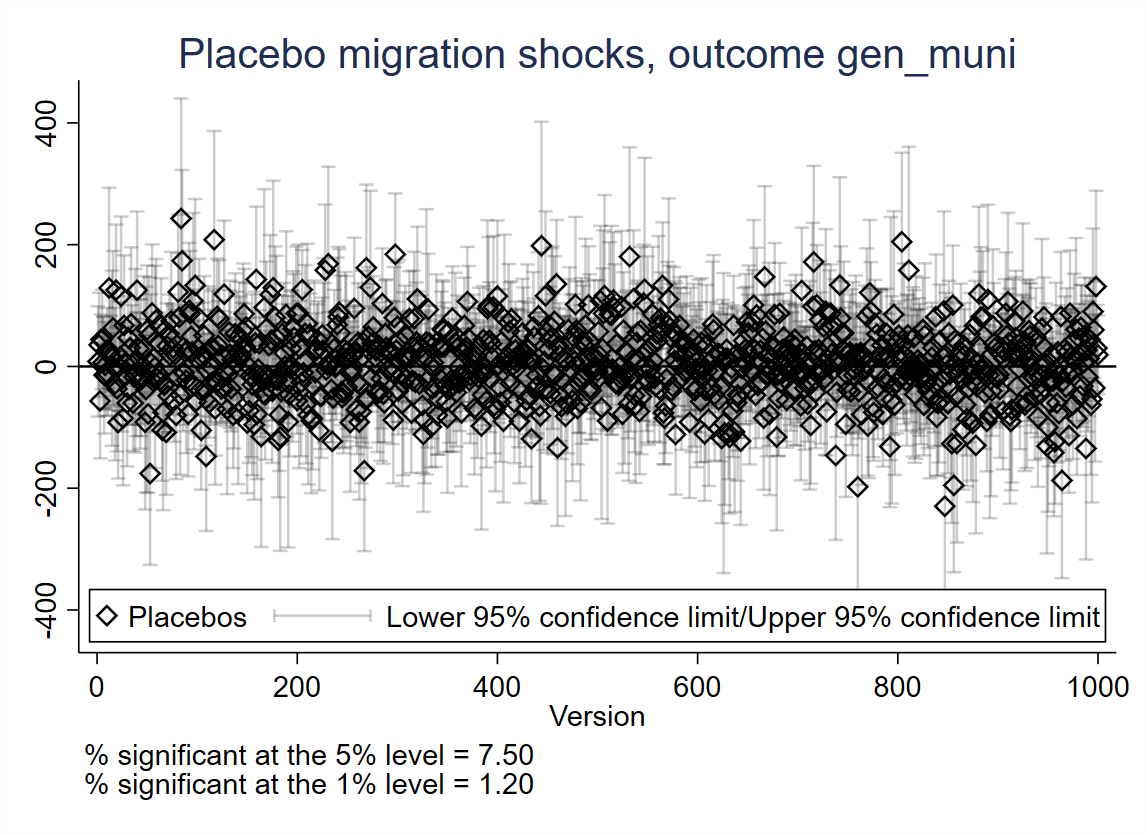
\includegraphics[width=\linewidth]{exhibits_old/figures/exogeneity_tests/D17_placebo_gen_muni_urban.png}
        % No caption here
        \label{fig:sub2}
    \end{subfigure}
    \begin{subfigure}{0.3\textwidth}
        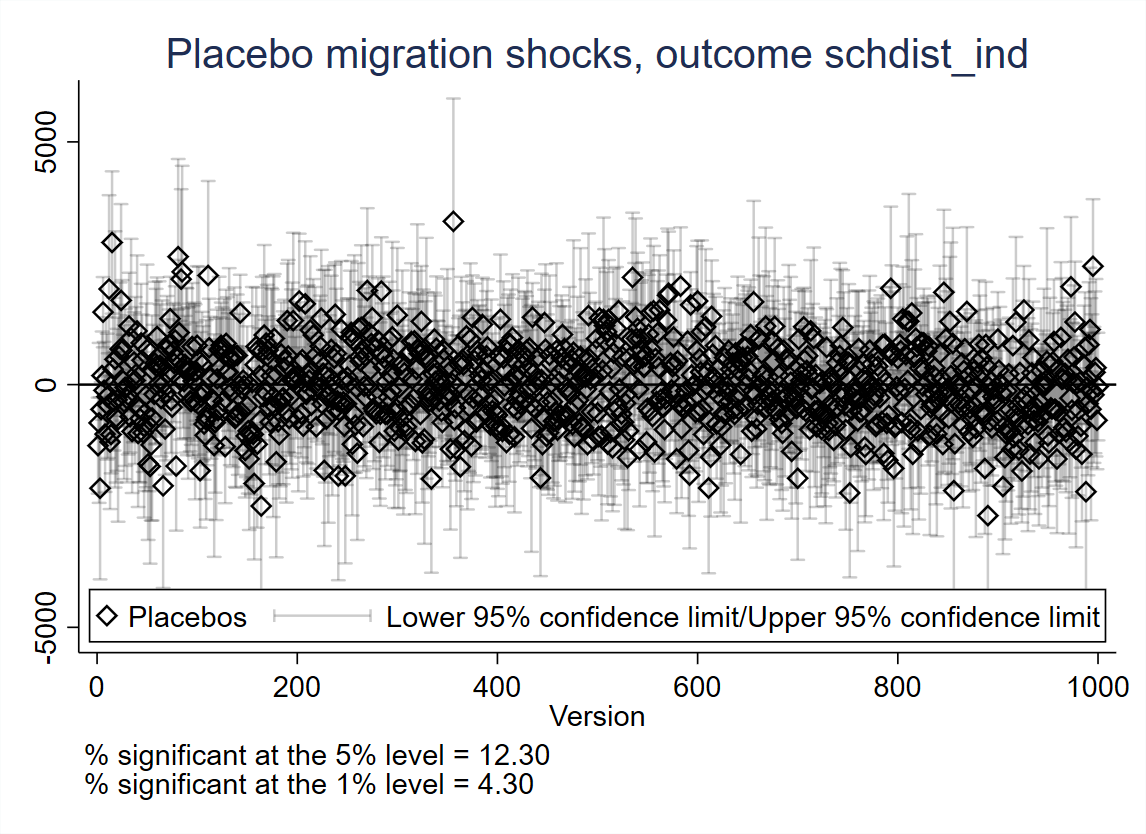
\includegraphics[width=\linewidth]{exhibits_old/figures/exogeneity_tests/D17_placebo_schdist_ind_urban.png}
        % No caption here
        \label{fig:sub3}
    \end{subfigure}

    \begin{subfigure}{0.3\textwidth}
        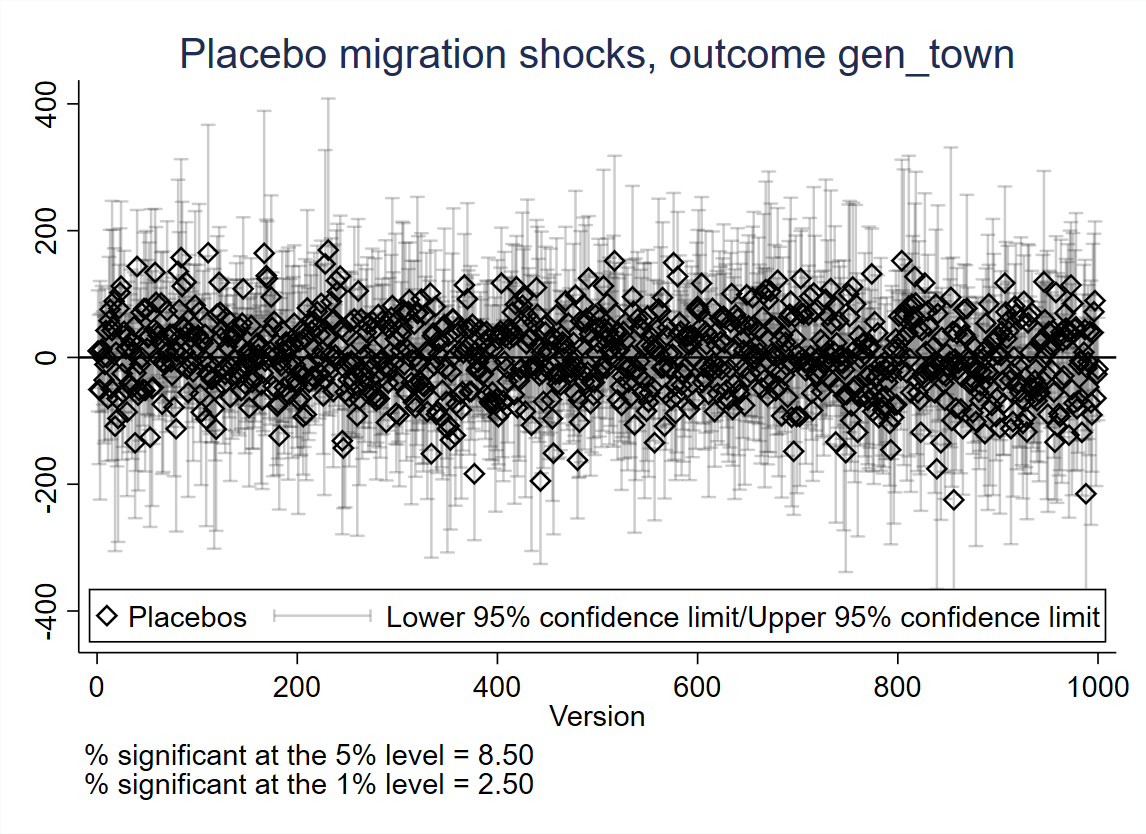
\includegraphics[width=\linewidth]{exhibits_old/figures/exogeneity_tests/D17_placebo_gen_town_urban.png}
        % No caption here
        \label{fig:sub4}
    \end{subfigure}
    \begin{subfigure}{0.3\textwidth}
        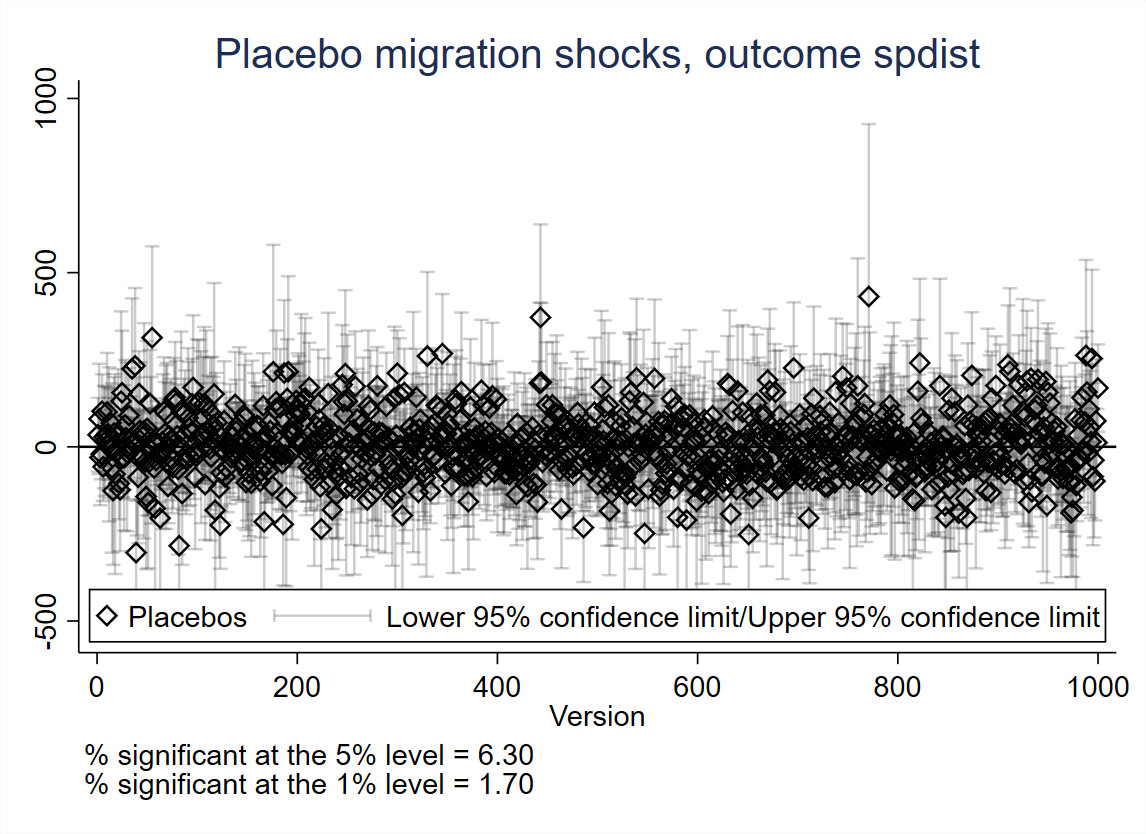
\includegraphics[width=\linewidth]{exhibits_old/figures/exogeneity_tests/D17_placebo_spdist_urban.png}
        % No caption here
        \label{fig:sub5}
    \end{subfigure}
    \caption{Placebo Test, Old}
    \label{fig:all}
\end{figure*}
\clearpage
\begin{figure*}[htbp]
    \centering
    \begin{subfigure}{0.3\textwidth}
        \includegraphics[width=\linewidth]{exhibits/figures/exogeneity_tests/D17_placebo_cgoodman_urban.png}
        % No caption here
        \label{fig:sub1}
    \end{subfigure}
    \begin{subfigure}{0.3\textwidth}
        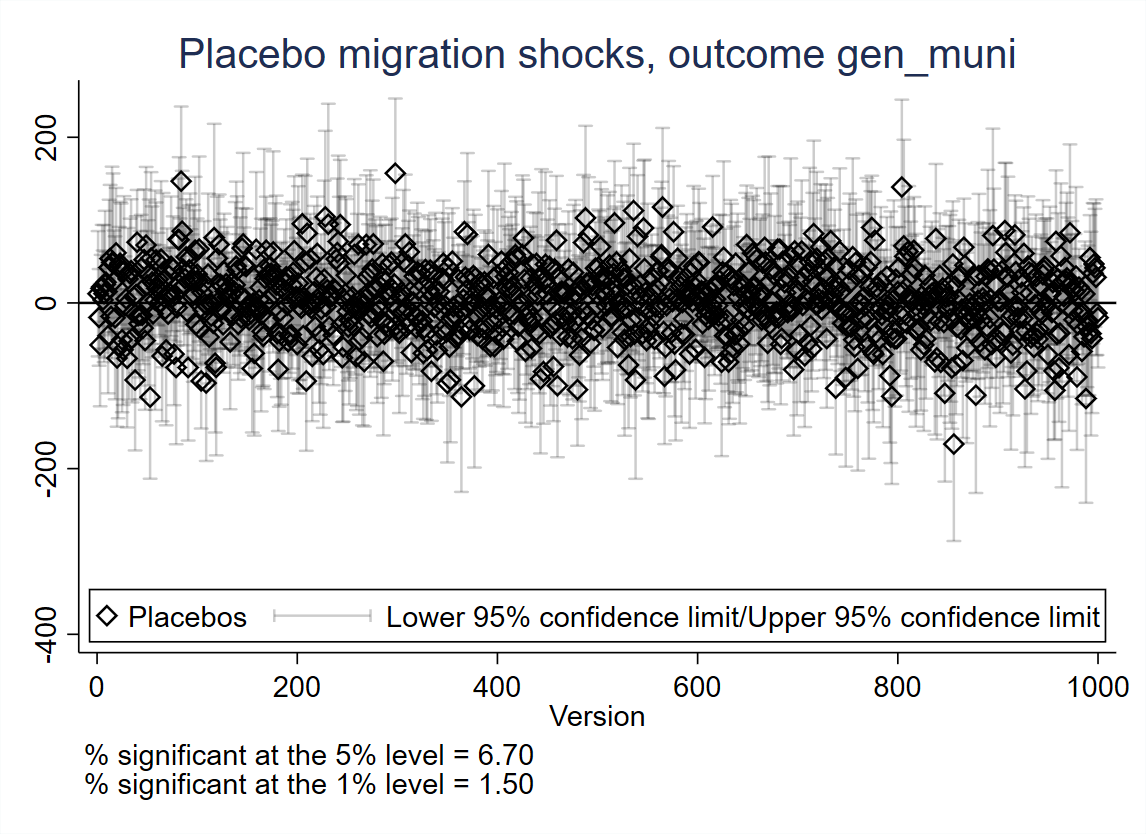
\includegraphics[width=\linewidth]{exhibits/figures/exogeneity_tests/D17_placebo_gen_muni_urban.png}
        % No caption here
        \label{fig:sub2}
    \end{subfigure}
    \begin{subfigure}{0.3\textwidth}
        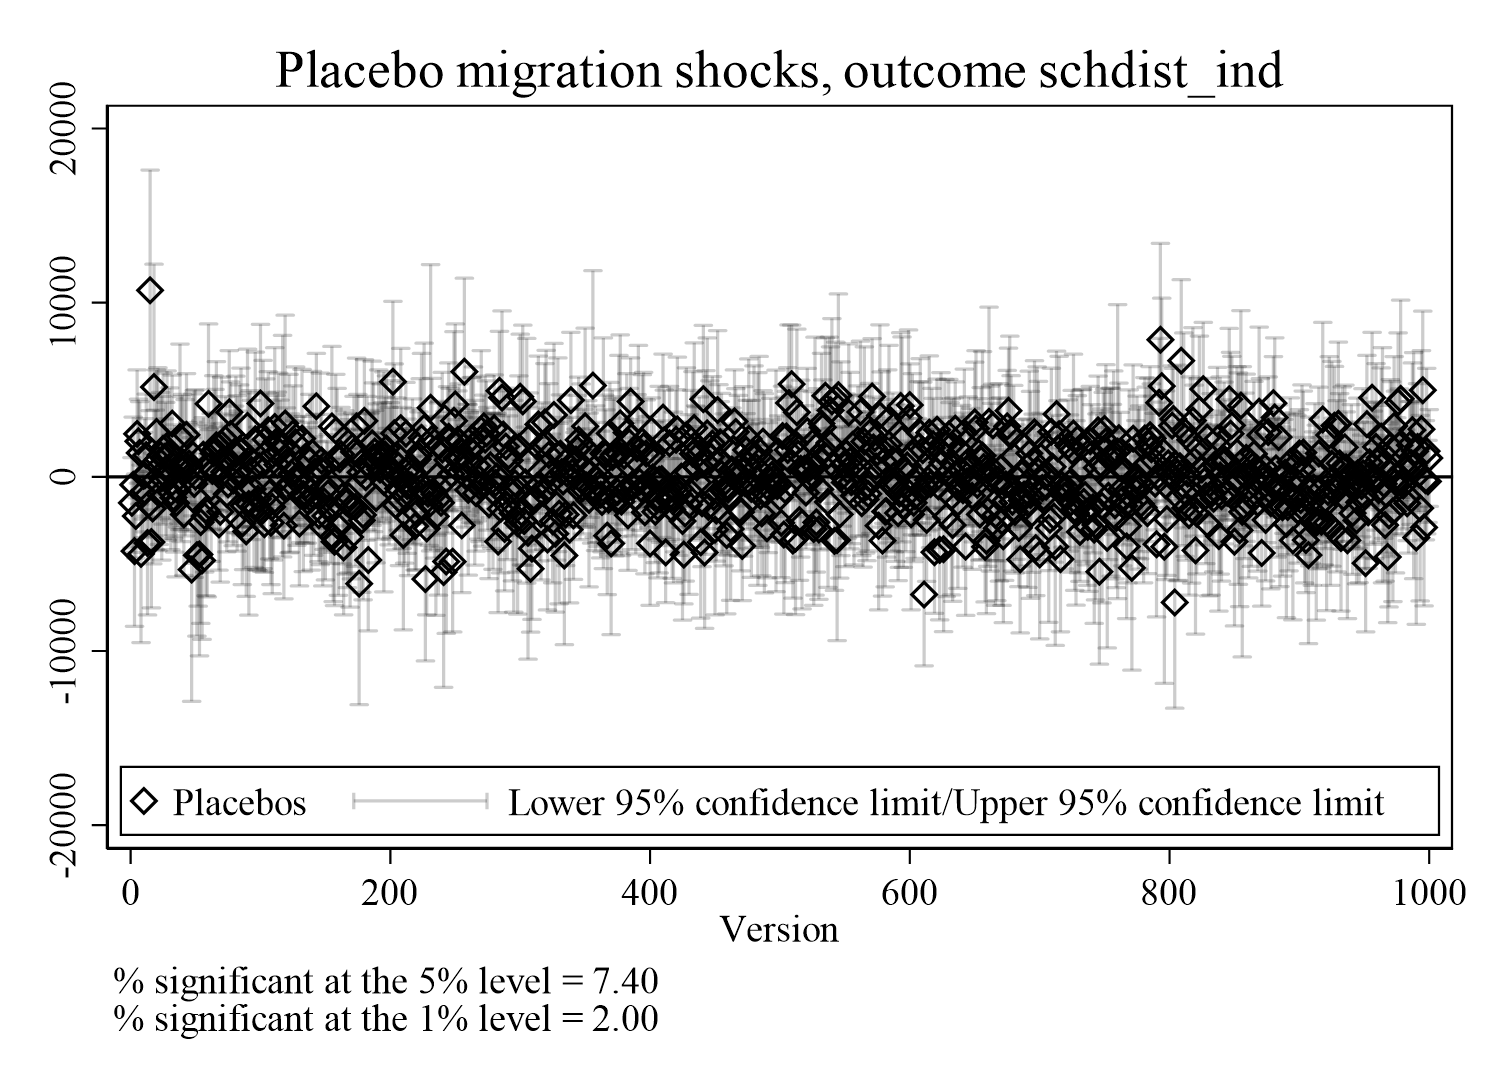
\includegraphics[width=\linewidth]{exhibits/figures/exogeneity_tests/D17_placebo_schdist_ind_urban.png}
        % No caption here
        \label{fig:sub3}
    \end{subfigure}

    \begin{subfigure}{0.3\textwidth}
        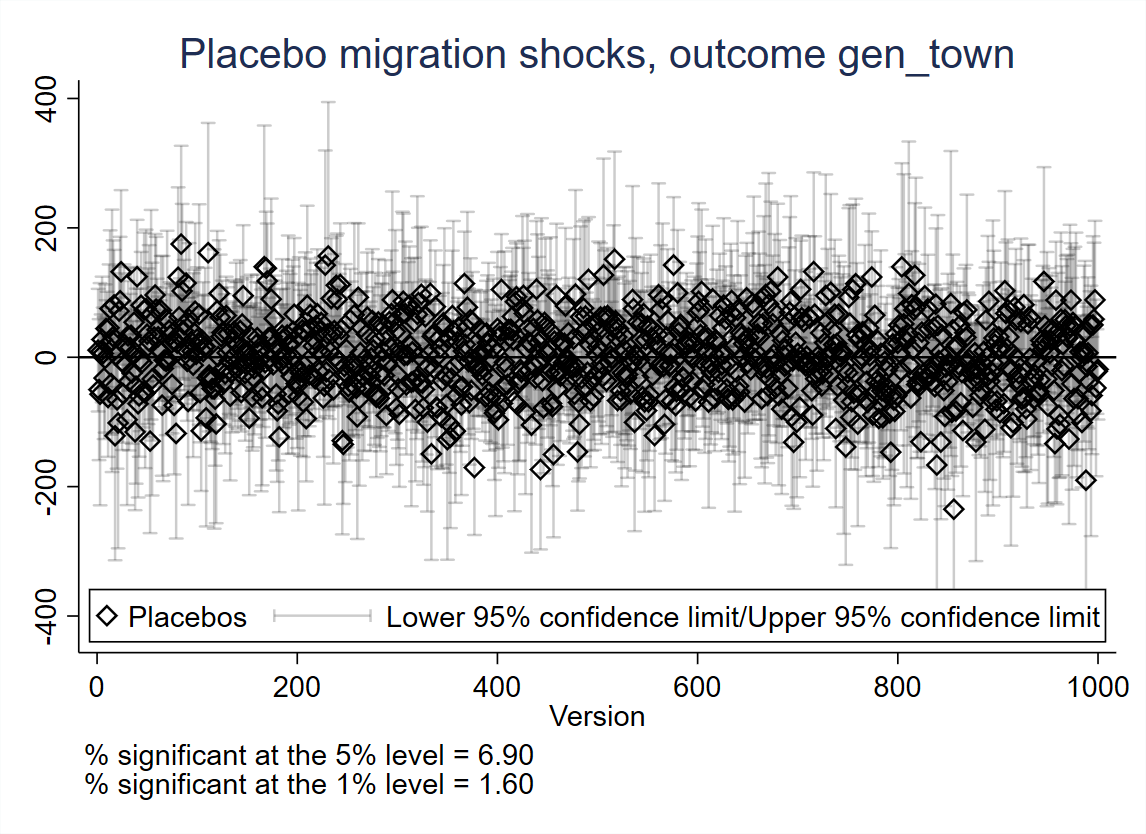
\includegraphics[width=\linewidth]{exhibits/figures/exogeneity_tests/D17_placebo_gen_town_urban.png}
        % No caption here
        \label{fig:sub4}
    \end{subfigure}
    \begin{subfigure}{0.3\textwidth}
        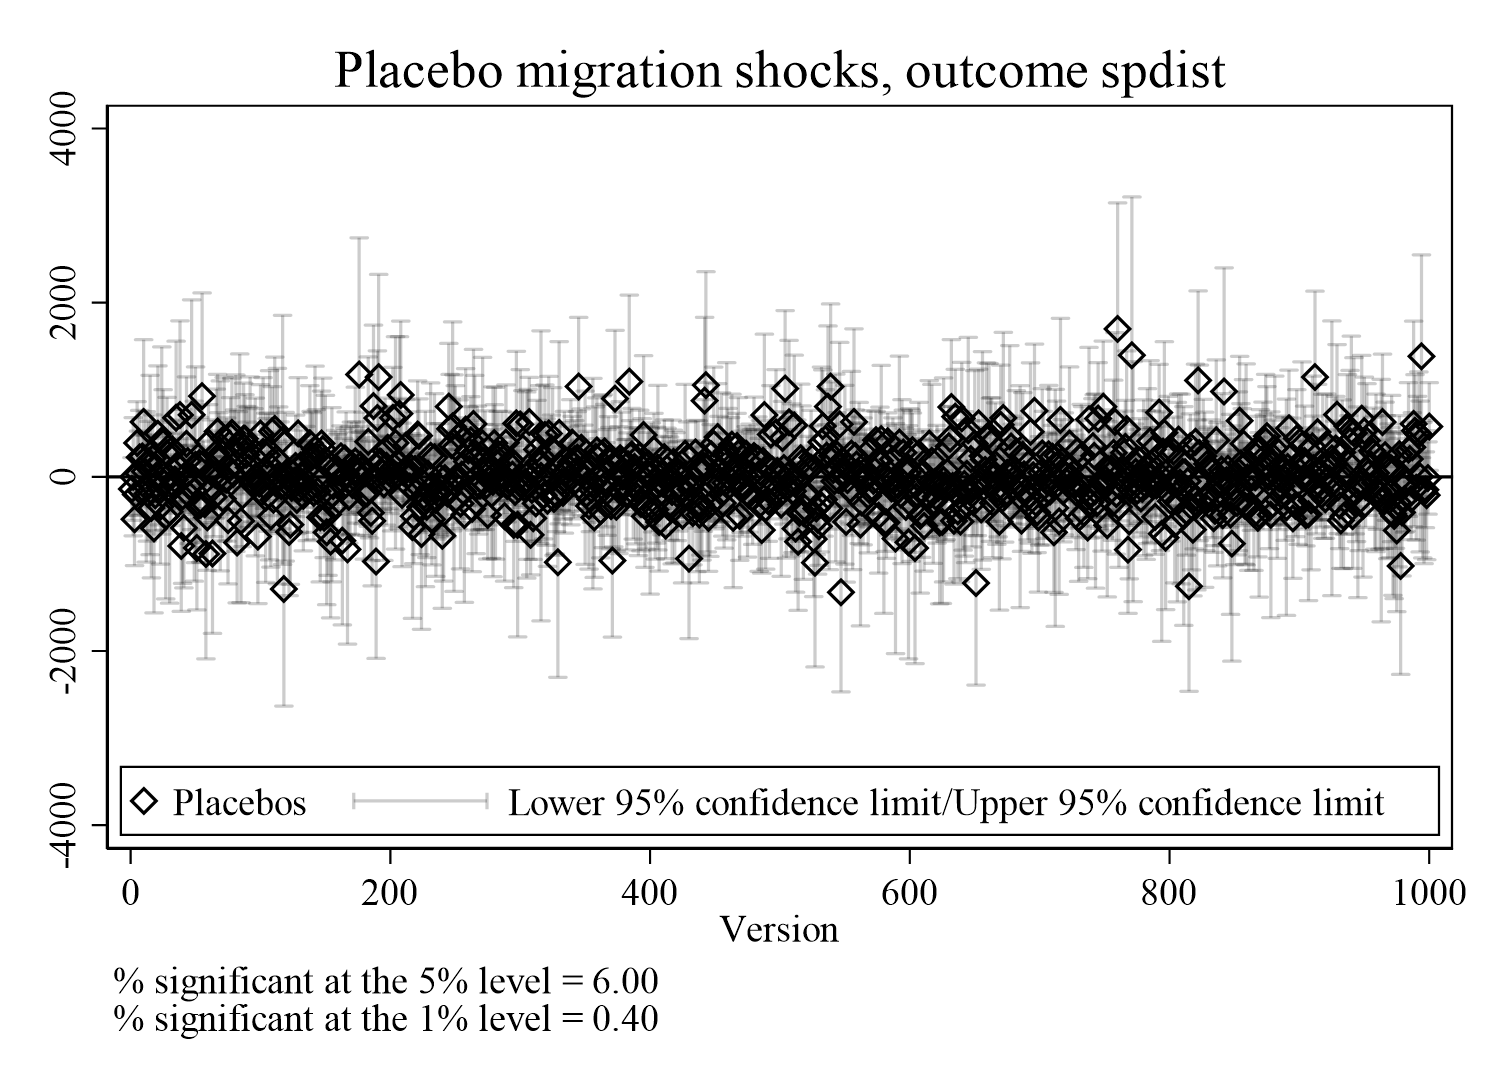
\includegraphics[width=\linewidth]{exhibits/figures/exogeneity_tests/D17_placebo_spdist_urban.png}
        % No caption here
        \label{fig:sub5}
    \end{subfigure}
    \begin{subfigure}{0.3\textwidth}
        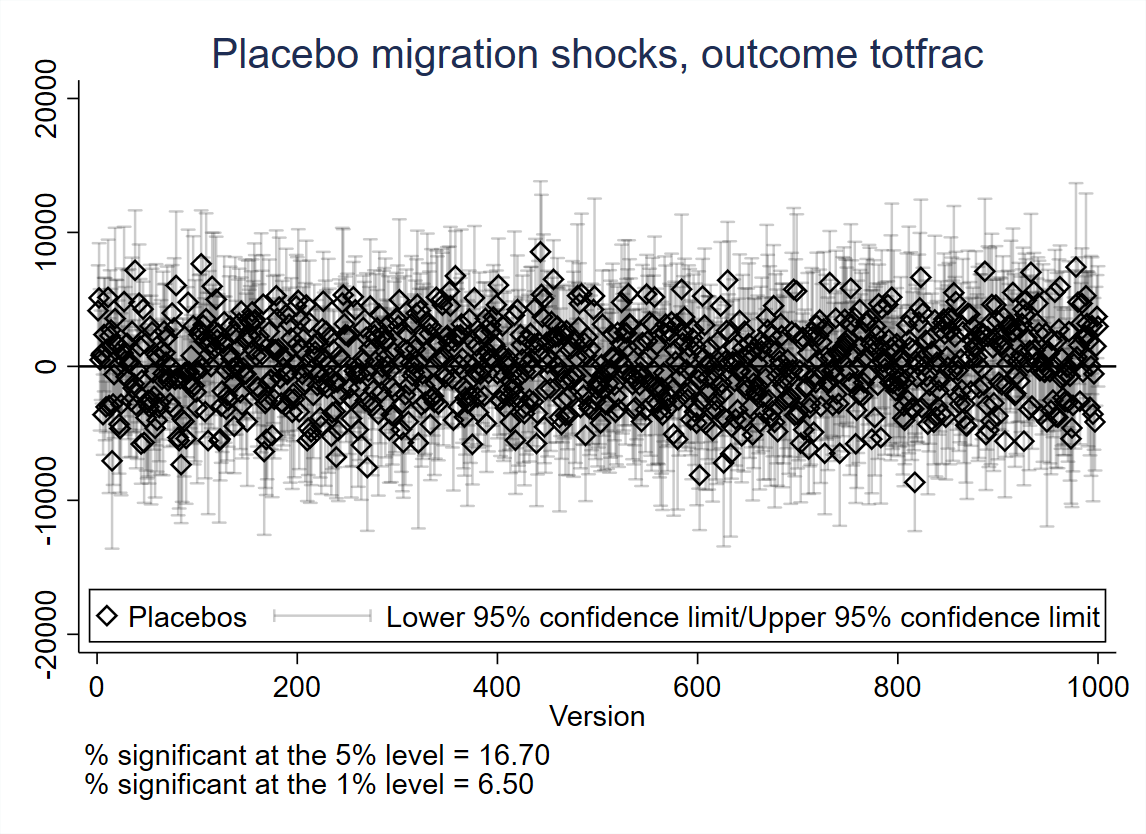
\includegraphics[width=\linewidth]{exhibits/figures/exogeneity_tests/D17_placebo_totfrac_urban.png}
        % No caption here
        \label{fig:sub6}
    \end{subfigure}

    \caption{Placebo Test, Updated}
    \label{fig:all}
\end{figure*}
\clearpage

\subsection{Alternative Instrument Tests}
\begin{figure*}[htbp]
    \centering
    \begin{subfigure}{0.3\textwidth}
        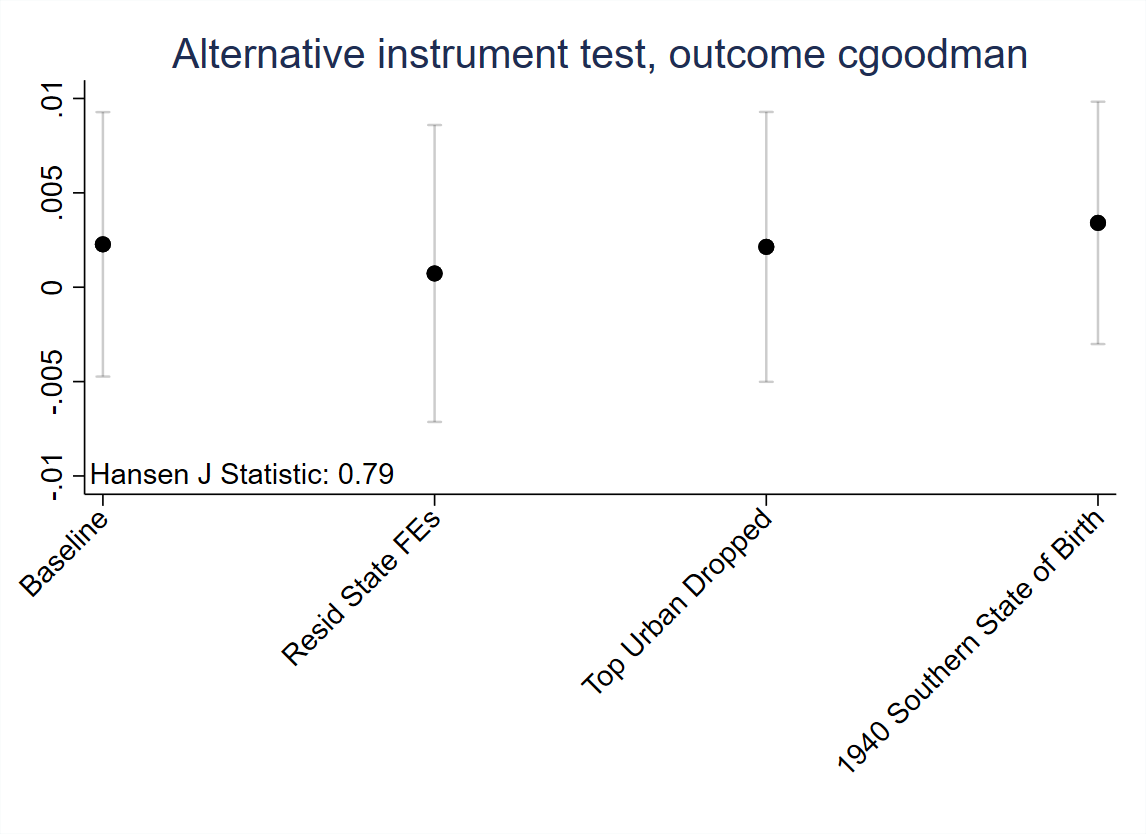
\includegraphics[width=\linewidth]{exhibits_old/figures/exogeneity_tests/D16_alt_inst_pooled_cgoodman.png}
        % No caption here
        \label{fig:sub1}
    \end{subfigure}
    \begin{subfigure}{0.3\textwidth}
        \includegraphics[width=\linewidth]{exhibits_old/figures/exogeneity_tests/D16_alt_inst_pooled_gen_muni.png}
        % No caption here
        \label{fig:sub2}
    \end{subfigure}
    \begin{subfigure}{0.3\textwidth}
        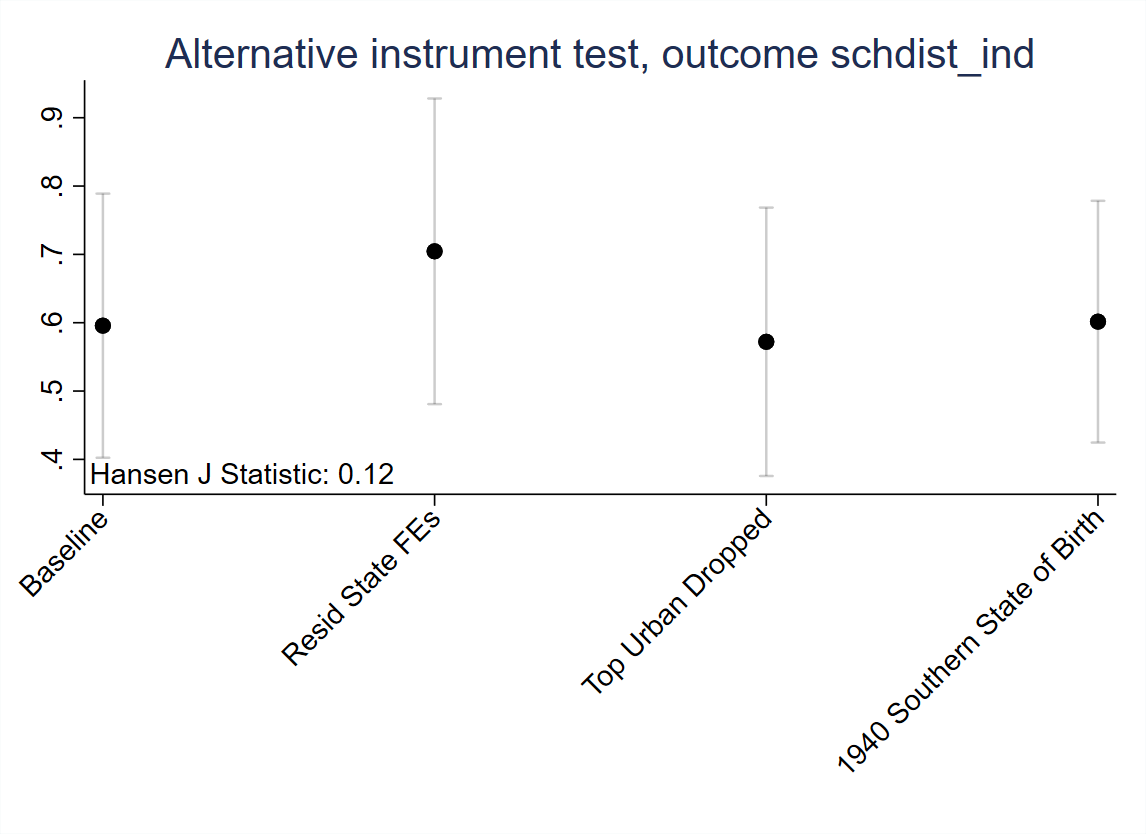
\includegraphics[width=\linewidth]{exhibits_old/figures/exogeneity_tests/D16_alt_inst_pooled_schdist_ind.png}
        % No caption here
        \label{fig:sub3}
    \end{subfigure}

    \begin{subfigure}{0.3\textwidth}
        \includegraphics[width=\linewidth]{exhibits_old/figures/exogeneity_tests/D16_alt_inst_pooled_gen_town.png}
        % No caption here
        \label{fig:sub4}
    \end{subfigure}
    \begin{subfigure}{0.3\textwidth}
        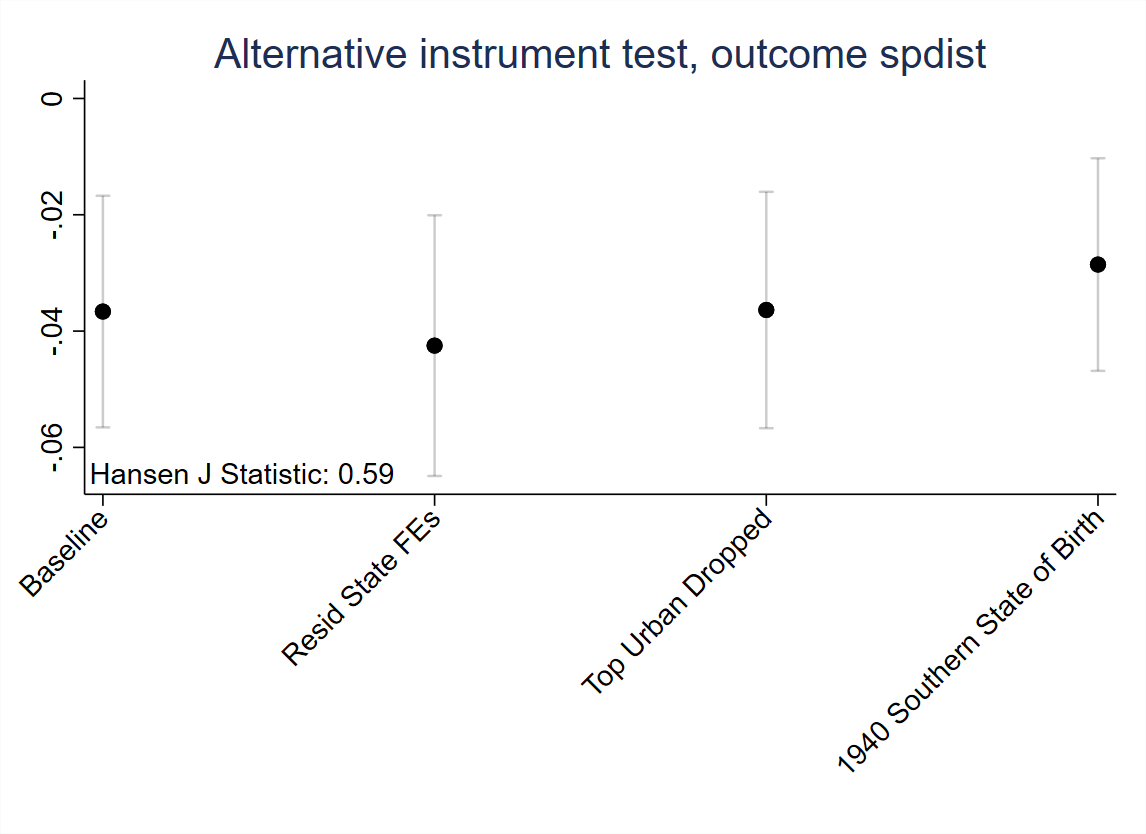
\includegraphics[width=\linewidth]{exhibits_old/figures/exogeneity_tests/D16_alt_inst_pooled_spdist.png}
        % No caption here
        \label{fig:sub5}
    \end{subfigure}
    \caption{Alternative Instrument Tests, Old}
    \label{fig:all}
\end{figure*}
\clearpage
\begin{figure*}[htbp]
    \centering
    \begin{subfigure}{0.3\textwidth}
        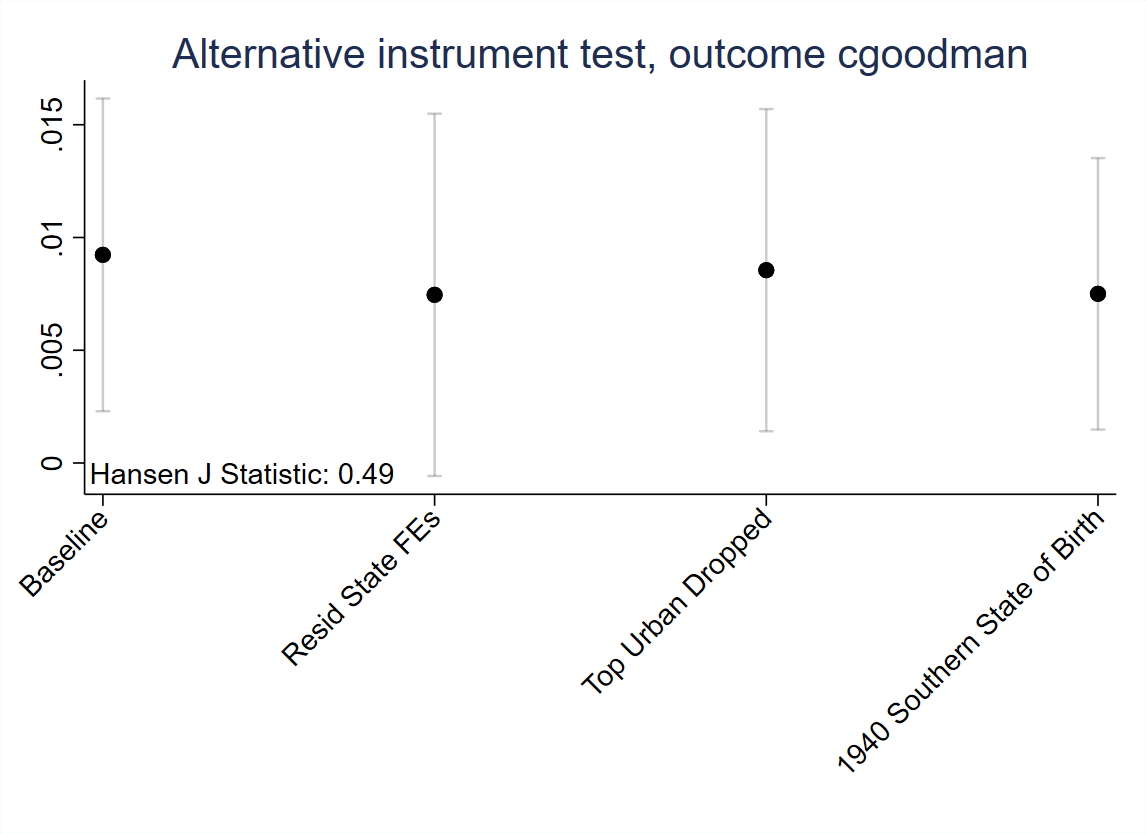
\includegraphics[width=\linewidth]{exhibits/figures/exogeneity_tests/D16_alt_inst_pooled_cgoodman.png}
        % No caption here
        \label{fig:sub1}
    \end{subfigure}
    \begin{subfigure}{0.3\textwidth}
        \includegraphics[width=\linewidth]{exhibits/figures/exogeneity_tests/D16_alt_inst_pooled_gen_muni.png}
        % No caption here
        \label{fig:sub2}
    \end{subfigure}
    \begin{subfigure}{0.3\textwidth}
        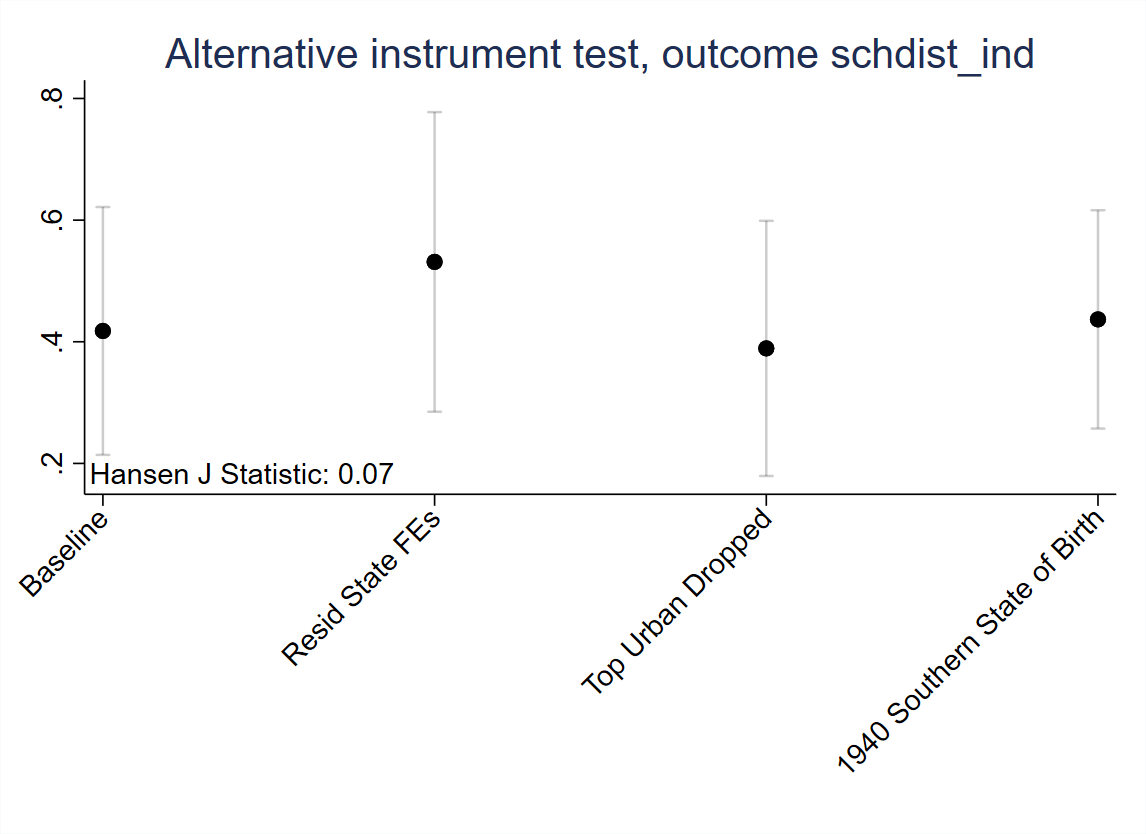
\includegraphics[width=\linewidth]{exhibits/figures/exogeneity_tests/D16_alt_inst_pooled_schdist_ind.png}
        % No caption here
        \label{fig:sub3}
    \end{subfigure}
    \begin{subfigure}{0.3\textwidth}
        \includegraphics[width=\linewidth]{exhibits/figures/exogeneity_tests/D16_alt_inst_pooled_gen_town.png}
        % No caption here
        \label{fig:sub5}
    \end{subfigure}
    \begin{subfigure}{0.3\textwidth}
        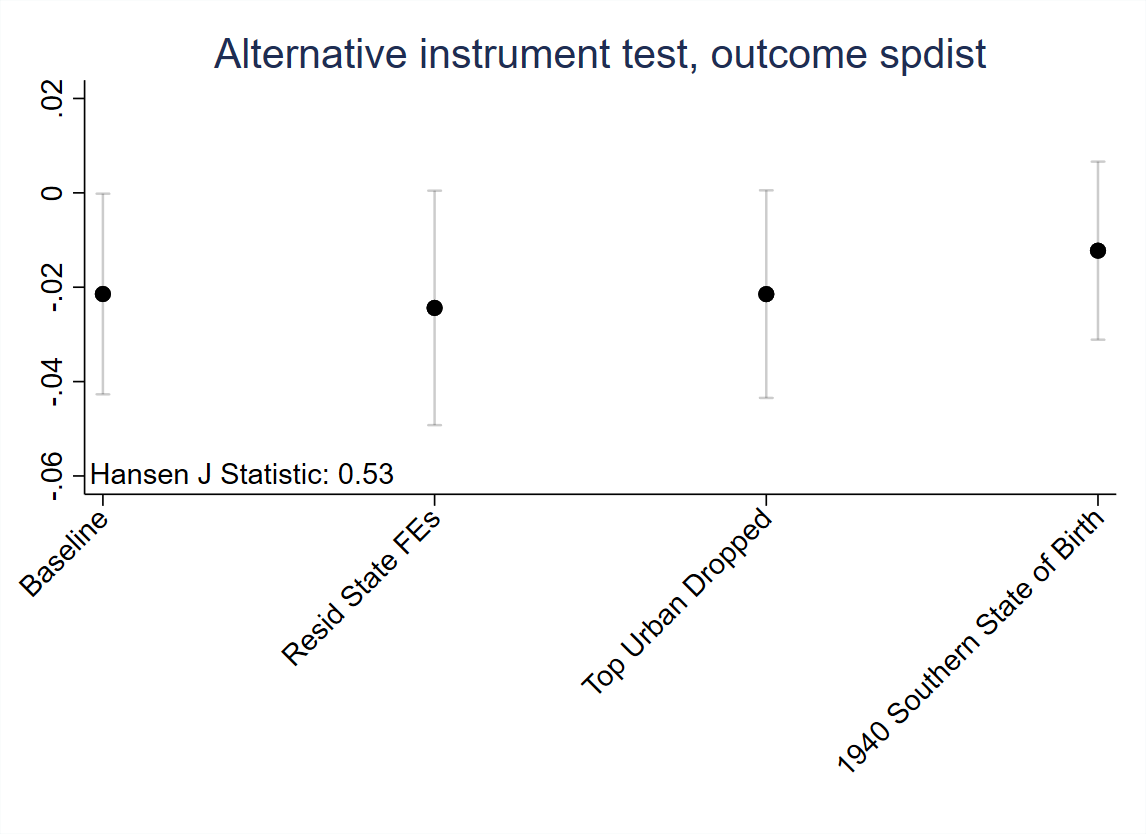
\includegraphics[width=\linewidth]{exhibits/figures/exogeneity_tests/D16_alt_inst_pooled_spdist.png}
        % No caption here
        \label{fig:sub6}
    \end{subfigure}
    \begin{subfigure}{0.3\textwidth}
        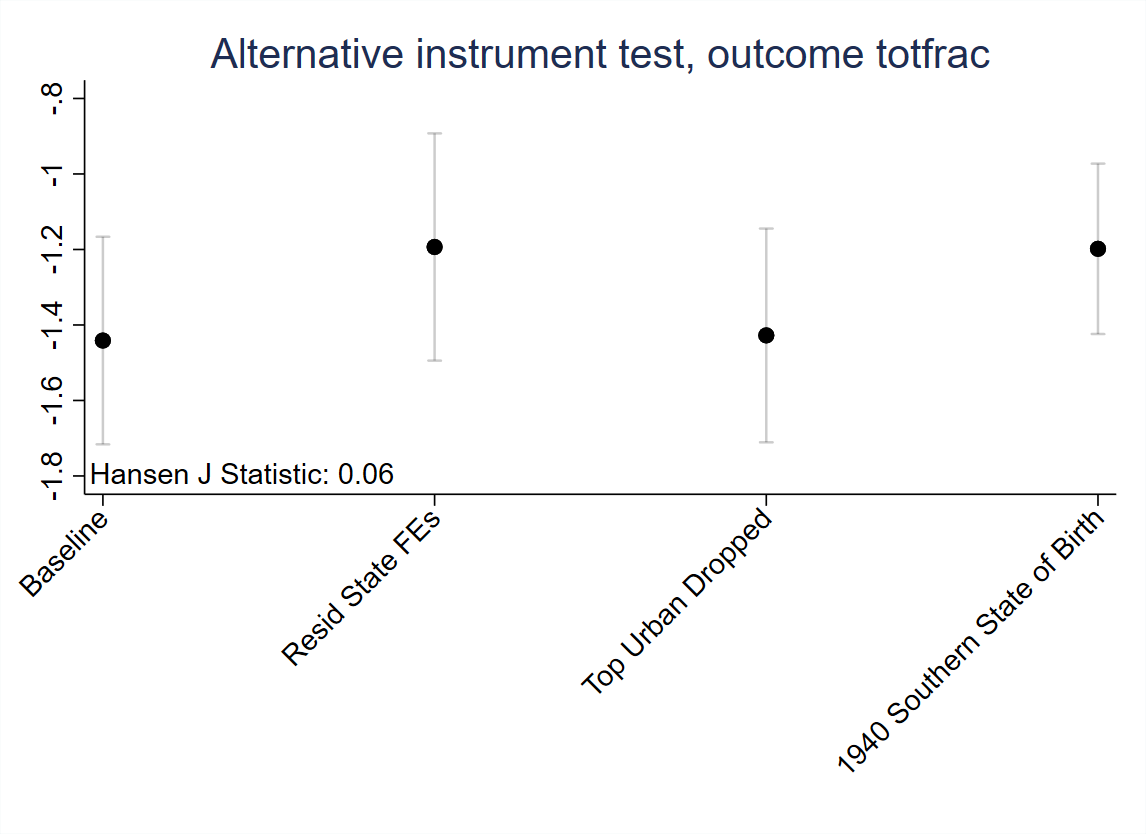
\includegraphics[width=\linewidth]{exhibits/figures/exogeneity_tests/D16_alt_inst_pooled_totfrac.png}
        % No caption here
        \label{fig:sub4}
    \end{subfigure}
    \caption{Alternative Instrument Tests, Updated}
    \label{fig:all}
\end{figure*}

\clearpage

\subsection{Leave-one-out Tests}
\begin{figure*}[htbp]
    \centering
    \begin{subfigure}{0.3\textwidth}
        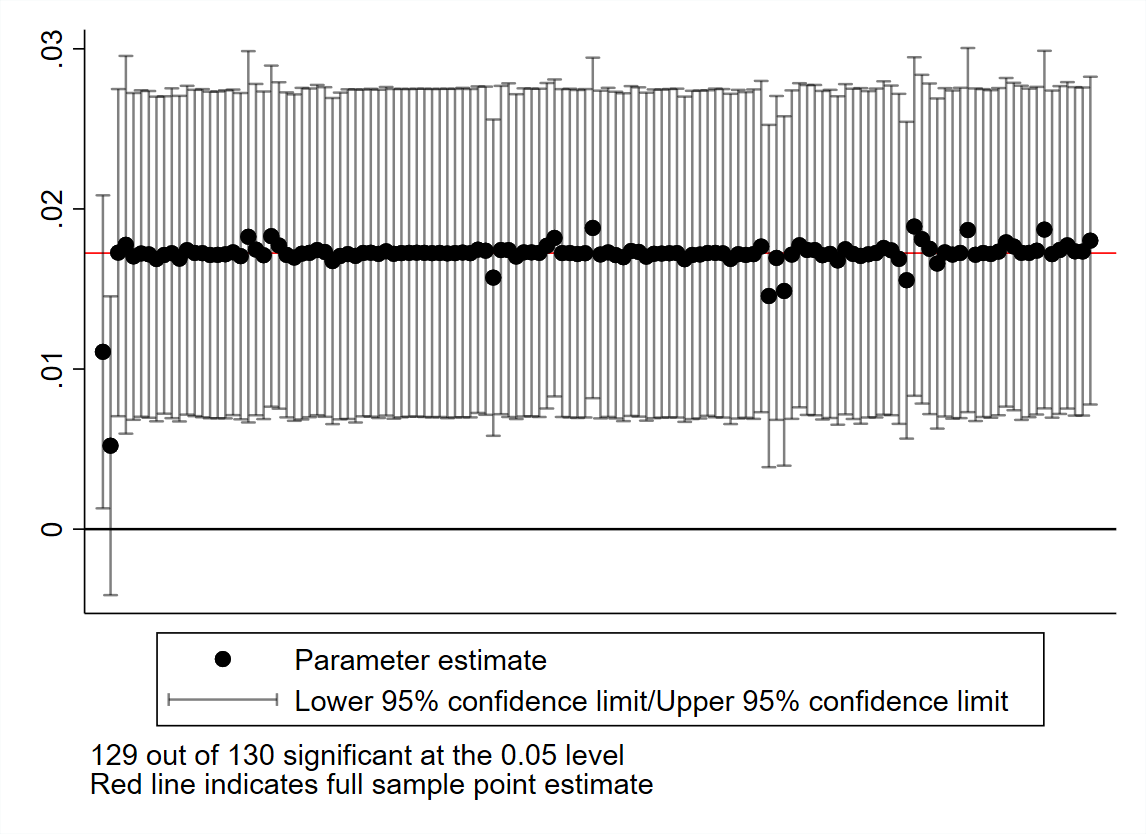
\includegraphics[width=\linewidth]{exhibits_old/figures/exogeneity_tests/loo_iv_cgoodman.png}
        % No caption here
        \label{fig:sub1}
    \end{subfigure}
    \begin{subfigure}{0.3\textwidth}
        \includegraphics[width=\linewidth]{exhibits_old/figures/exogeneity_tests/loo_iv_gen_muni.png}
        % No caption here
        \label{fig:sub2}
    \end{subfigure}
    \begin{subfigure}{0.3\textwidth}
        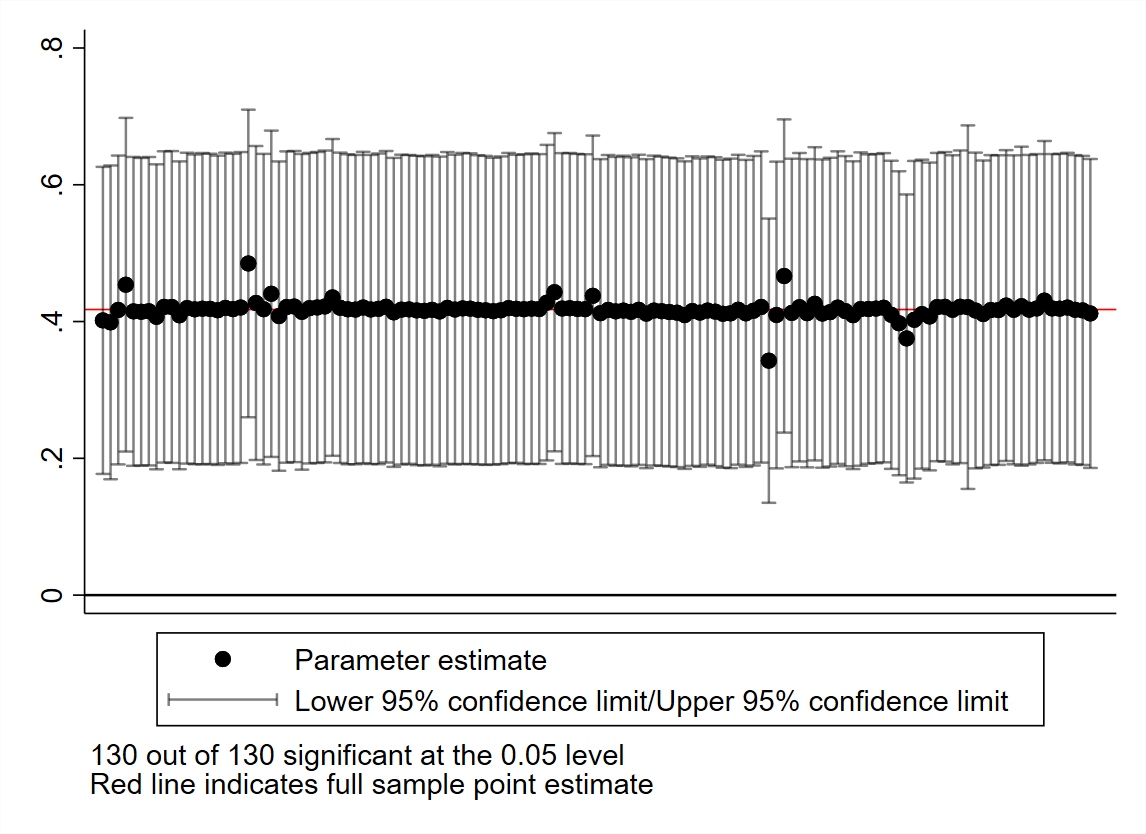
\includegraphics[width=\linewidth]{exhibits_old/figures/exogeneity_tests/loo_iv_schdist_ind.png}
        % No caption here
        \label{fig:sub3}
    \end{subfigure}

    \begin{subfigure}{0.3\textwidth}
        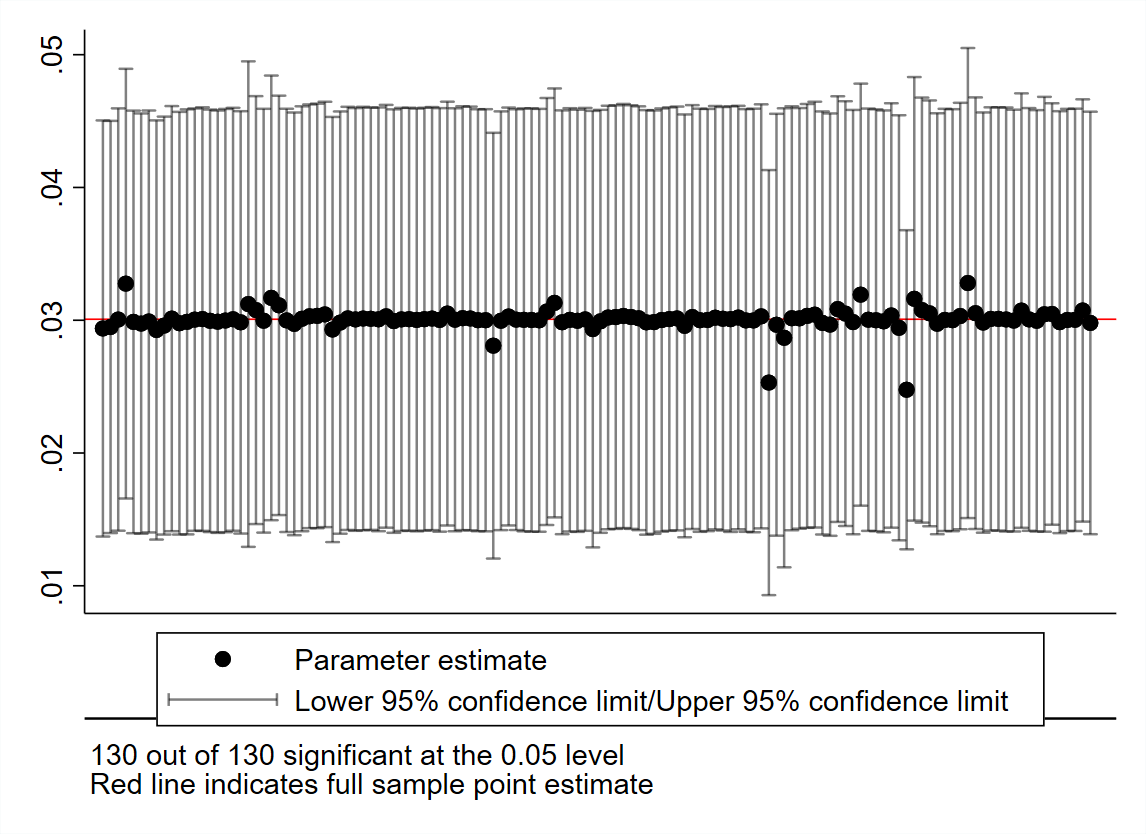
\includegraphics[width=\linewidth]{exhibits_old/figures/exogeneity_tests/loo_iv_gen_town.png}
        % No caption here
        \label{fig:sub4}
    \end{subfigure}
    \begin{subfigure}{0.3\textwidth}
        \includegraphics[width=\linewidth]{exhibits_old/figures/exogeneity_tests/loo_iv_spdist.png}
        % No caption here
        \label{fig:sub5}
    \end{subfigure}
    \caption{Leave-one-out IV Tests, Old}
    \label{fig:all}
\end{figure*}
\clearpage
\begin{figure*}[htbp]
    \centering
    \begin{subfigure}{0.3\textwidth}
        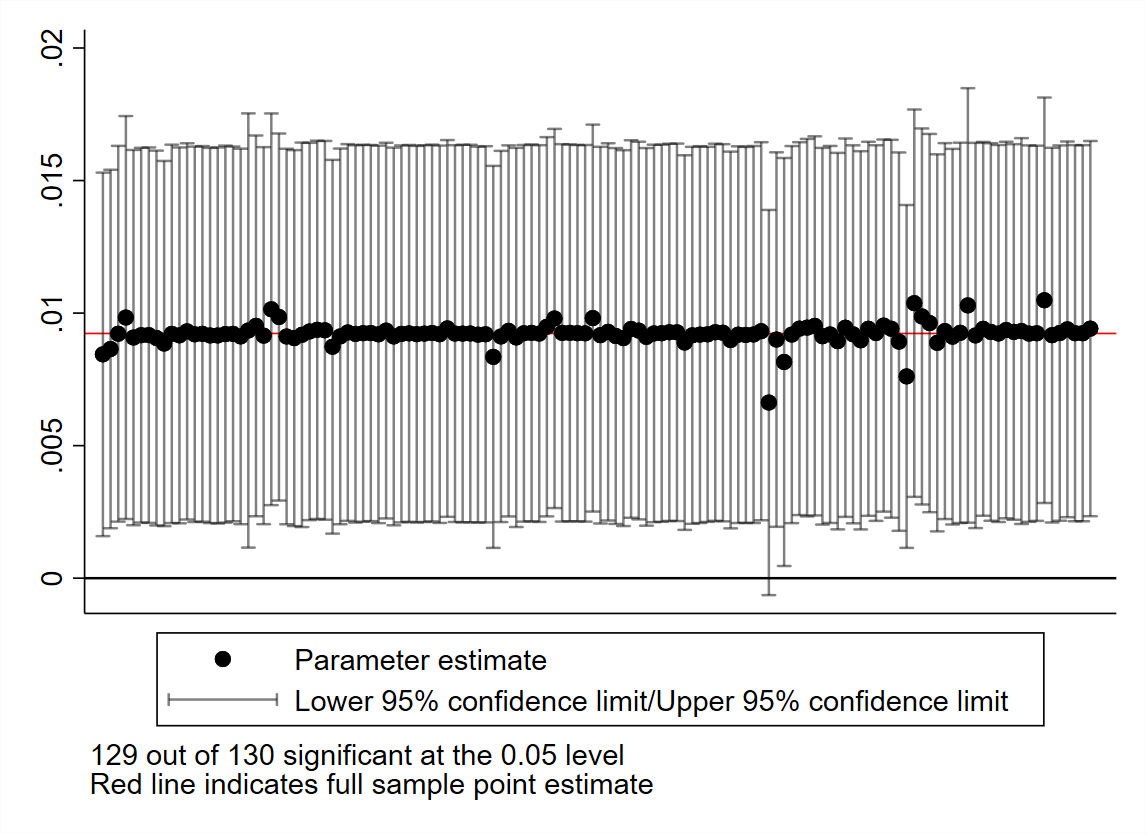
\includegraphics[width=\linewidth]{exhibits/figures/exogeneity_tests/loo_iv_cgoodman.png}
        % No caption here
        \label{fig:sub1}
    \end{subfigure}
    \begin{subfigure}{0.3\textwidth}
        \includegraphics[width=\linewidth]{exhibits/figures/exogeneity_tests/loo_iv_gen_muni.png}
        % No caption here
        \label{fig:sub2}
    \end{subfigure}
    \begin{subfigure}{0.3\textwidth}
        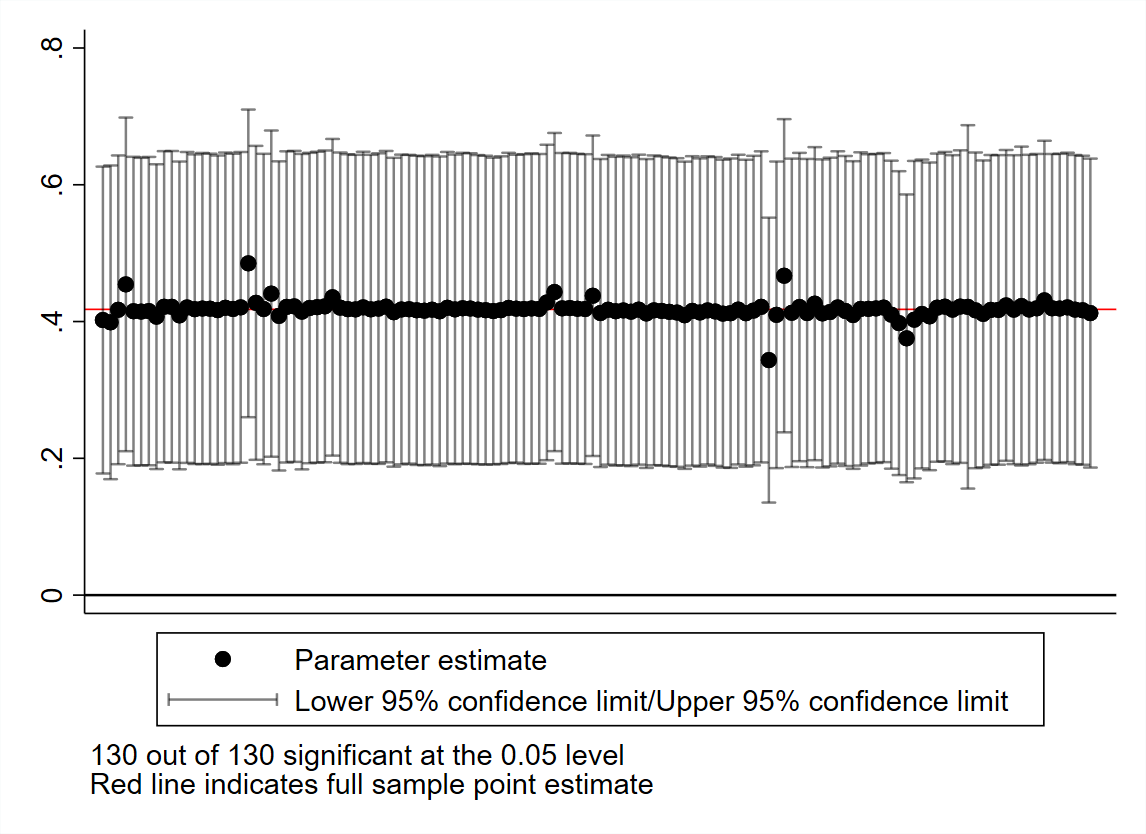
\includegraphics[width=\linewidth]{exhibits/figures/exogeneity_tests/loo_iv_schdist_ind.png}
        % No caption here
        \label{fig:sub3}
    \end{subfigure}
    \begin{subfigure}{0.3\textwidth}
        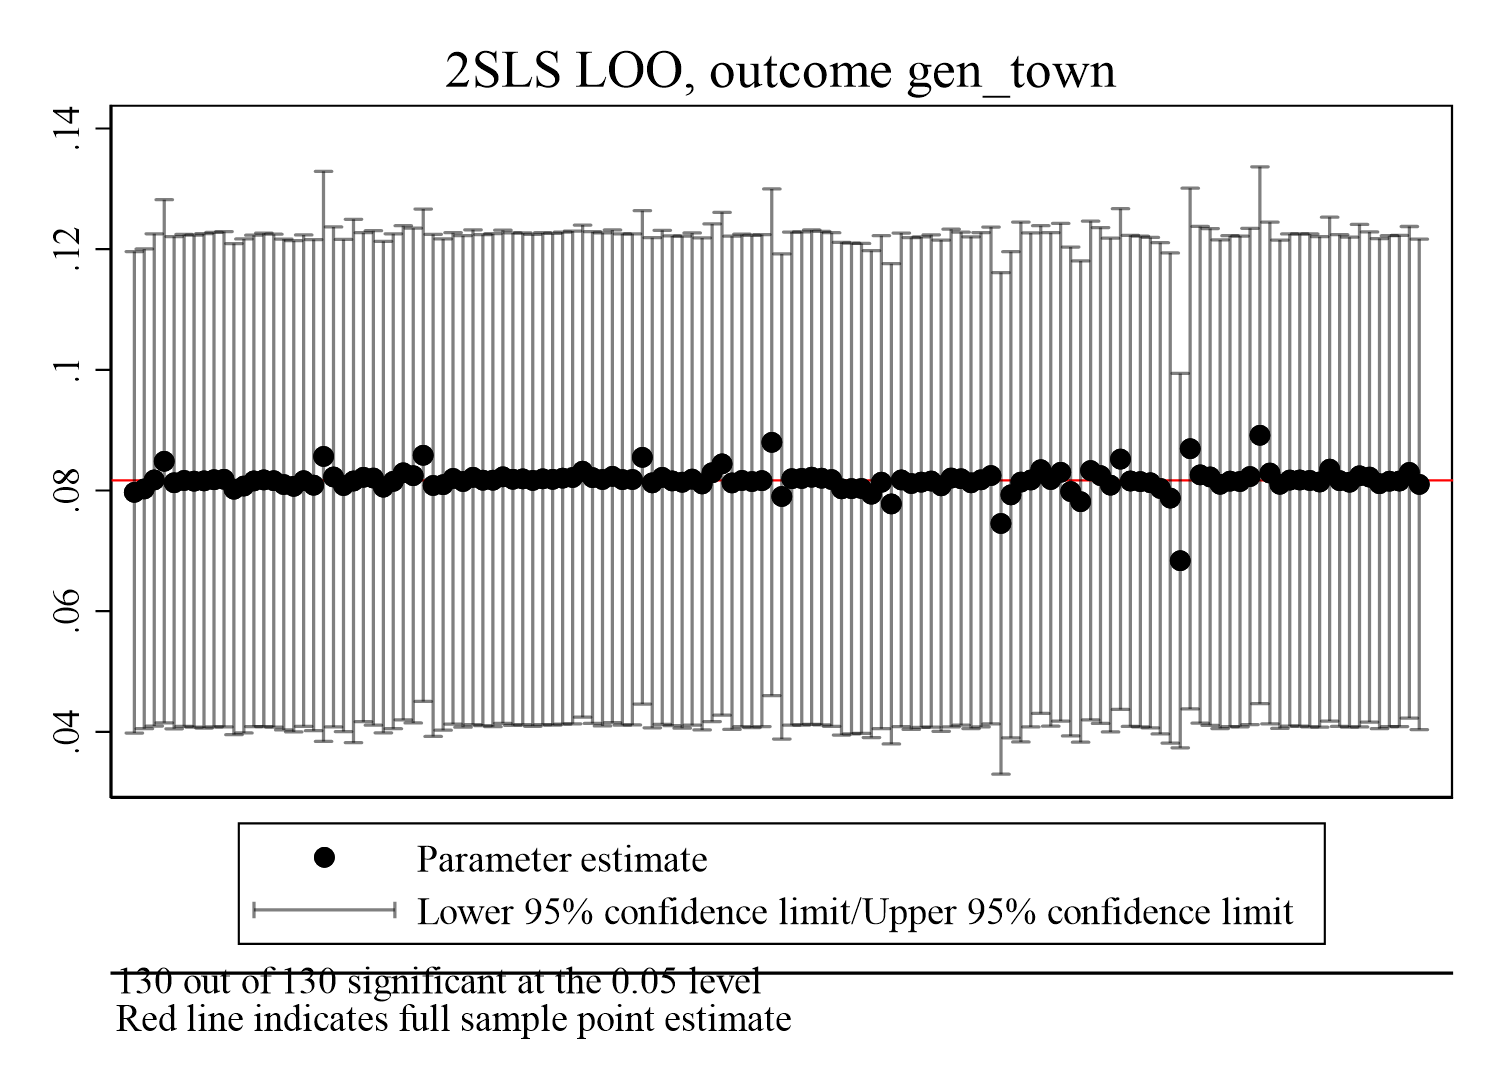
\includegraphics[width=\linewidth]{exhibits/figures/exogeneity_tests/loo_iv_gen_town.png}
        % No caption here
        \label{fig:sub5}
    \end{subfigure}
    \begin{subfigure}{0.3\textwidth}
        \includegraphics[width=\linewidth]{exhibits/figures/exogeneity_tests/loo_iv_spdist.png}
        % No caption here
        \label{fig:sub6}
    \end{subfigure}
    \begin{subfigure}{0.3\textwidth}
        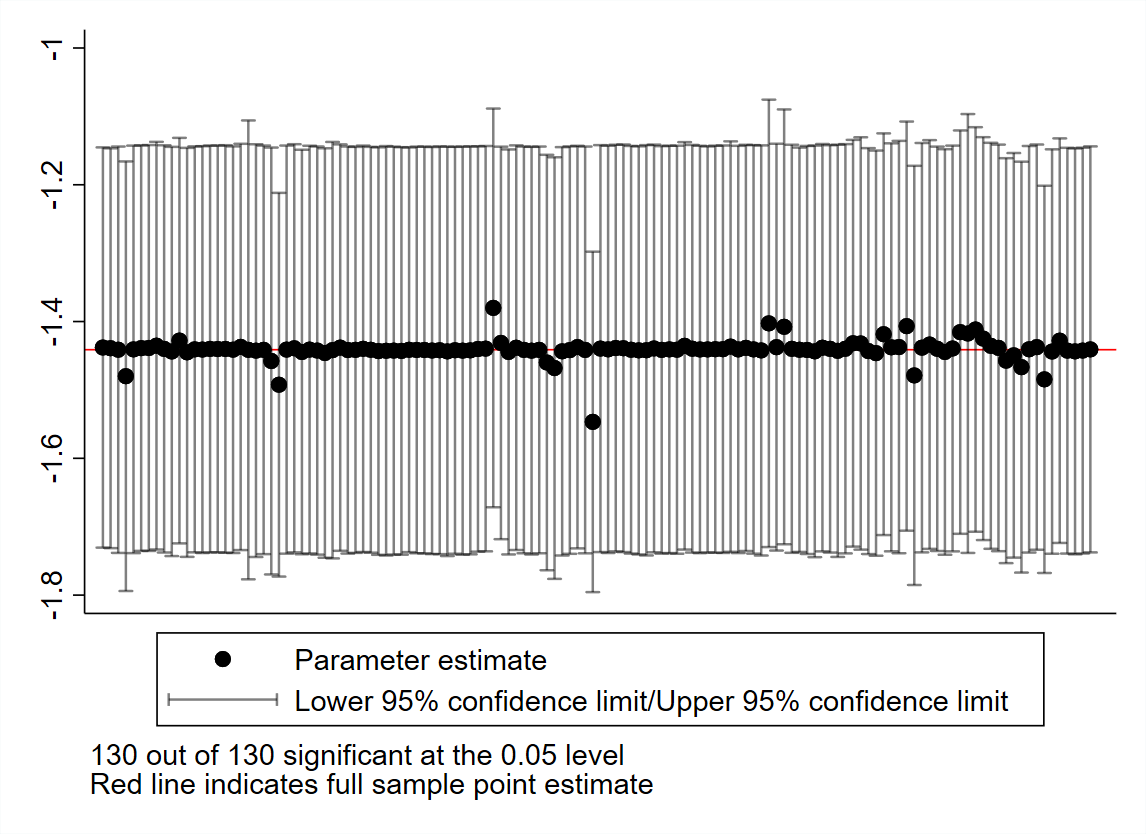
\includegraphics[width=\linewidth]{exhibits/figures/exogeneity_tests/loo_iv_totfrac.png}
        % No caption here
        \label{fig:sub4}
    \end{subfigure}
    \caption{Leave-one-out IV Tests, Updated}
    \label{fig:all}
\end{figure*}
\end{document}